\documentclass[12pt,a4paper,openright,twoside]{book}
\usepackage[utf8]{inputenc}
\usepackage{amsmath}
\usepackage{amssymb}
\usepackage{listings}
\usepackage{algorithm}
\usepackage{algpseudocode}
\usepackage{tabularx}
\usepackage{graphicx}
\usepackage{disi-thesis}
\usepackage{code-lstlistings}
\usepackage{notes}
\usepackage{shortcuts}
\usepackage{acronym}
\usepackage{tikz}
\usepackage{float}
\usepackage{pgfplots}
\pgfplotsset{width=10cm,compat=1.9}
%\usepackage[linesnumbered,ruled,vlined]{algorithm2e}

\usetikzlibrary{shapes.geometric, arrows}
\graphicspath{{./sections/}}

\newcommand{\thesislang}{english} % commentare in caso di tesi in italiano
%\usepackage{thesis-style}
% version
%\newcommand{\versionmajor}{0}
%\newcommand{\versionminor}{1}
%\newcommand{\versionpatch}{2}
%\newcommand{\version}{\versionmajor.\versionminor.\versionpatch}
%\typeout{Document version: \version}

\school{\unibo}
\programme{Corso di Laurea Magistrale in Ingegneria e Scienze Informatiche}
\title{Fair-by-design algoriths for access to education}
\author{Antonio Iannotta}
\date{\today}
\subject{Intelligent Systems Engineering}
\supervisor{Prof. Giovanni Ciatto}
\cosupervisor{Prof. Roberta Calegari}
\morecosupervisor{Prof. Andrea Omicini}
\session{IV}
\academicyear{2022-2023}

% Definition of acronyms
\acrodef{IoT}{Internet of Thing}
\acrodef{vm}[VM]{Virtual Machine}
\acrodef{AI}{Artificial Intelligence}

\tikzstyle{startstop} = [rectangle, rounded corners, 
minimum width=3cm, 
minimum height=1cm,
text centered, 
draw=black, 
fill=blue!30]

\tikzstyle{decision} = [diamond, 
minimum width=3cm, 
minimum height=1cm, 
text centered, 
draw=black, 
fill=green!30]

\tikzstyle{arrow} = [thick,->,>=stealth]

\mainlinespacing{1.241} % line spacing in mainmatter, comment to default

\begin{document}
	
\frontmatter
% ! TeX root = thesis-main.tex
\title{Title}
\author{Candidate Name Here}
\date{\today}

\newgeometry{margin=0.8in}
\begin{titlepage}
	\begin{center}
		% \vspace*{0.2cm}
		
		\large
		\textbf{ALMA MATER STUDIORUM -- UNIVERSITÀ DI BOLOGNA \\ CAMPUS DI CESENA}
		\\
		\noindent\hrulefill
		\vspace{0.4cm}
		
		\Large
		Scuola di Ingegneria e Architettura \\
		Corso di Laurea Magistrale in Ingegneria e Scienze Informatiche
		
		\Huge
		\vspace{4cm}
		\textbf{
			Fair-by-design algorithm for access to education
		}
		
		\large
		\vspace{1cm}
		Tesi di laurea in 
		\\
		\textsc{Intelligent Systems Engineering}
		
		\vspace{5.5cm}
		\begin{minipage}[t]{0.64\textwidth}
			\begin{flushleft}
				\textit{Relatore} 
				\\ 
				\textbf{Prof.} \textbf{Giovanni Ciatto}
				\\
				\vspace{0.4cm}
				\textit{Correlatore} 
				\\
				\textbf{Prof.} \textbf{Roberta Calegari}
				\\
				\textbf{Prof.} \textbf{Andrea Omicini}
			\end{flushleft}
		\end{minipage}
		\begin{minipage}[t]{0.34\textwidth}
			\begin{flushright}
				\textit{Candidato} 
				\\ 
				\textbf{Antonio Iannotta}
			\end{flushright}
		\end{minipage}\\
		
		\vfill
		\noindent\hrulefill
		\vspace{0.3cm}
		\Large
		
		IV Sessione di Laurea
		\\
		Anno Accademico 2022/2023
	\end{center}
\end{titlepage}
\restoregeometry


\begin{abstract}

    This work presents an in-depth approach to address fairness and bias mitigation in the design and development of data-driven methods. The primary contribution of this study is the proposal and implementation of an innovative \emph{Fair-by-Design} workflow that incorporates various strategies for bias mitigation within data, algorithms, and decision-making processes.

    The work focuses on the educational data of the Canary Islands, leveraging a dataset encompassing detailed information about student performance and educational outcomes.

    The primary objective is to ensure equitable and unbiased application of data-driven algorithms within the educational context. 

    The methodology involves the systematic evaluation of multiple bias mitigation strategies. The critical aspect of this research centers on the comparison of these strategies based on their impact on the predictive accuracy of the algorithms. 

    This approach provides practical insights into the trade-offs between fairness and accuracy, showing how several approaches can lead to different accuracy scores on the same dataset and with the same models. 

    The work findings offer valuable insights into the trade-offs between fairness and accuracy when developing data-driven methods for educational data. 

    This thesis contributes to the ongoing discourse on fairness in machine learning and data-driven decision-making. The results provide guidance for stakeholders in the education sector, aiding them in making informed decisions about algorithm deployment to promote fairness and minimize bias within educational systems. 

\end{abstract}
    

%\begin{acknowledgements} % this is optional
%Never too far down, to come back
%\end{acknowledgements}

%----------------------------------------------------------------------------------------
\tableofcontents   
\listoffigures     % (optional) comment if empty
%\lstlistoflistings % (optional) comment if empty
%----------------------------------------------------------------------------------------

\mainmatter

\chapter{Introduction}
\label{chap:introduction}

Artificial Intelligence (AI) has experienced an unprecedented surge in prominence and utility in recent years, emerging as a transformative force across diverse domains. From powering autonomous vehicles to aiding healthcare diagnosis and recommendation systems, AI applications have become increasingly woven into the fabric of daily lives. However, this rapid proliferation has ushered in a pressing concern about the pervasive presence of bias within AI systems.

The concept of bias in AI pertains to the inadvertent or systematic preference shown towards specific groups or characteristics within the data, algorithms, or decision-making processes. This partiality leads to outcomes that are unjust, unfair, and unequal. In this era of AI-driven decision-making, the imperative to address bias is not just a technological challenge but a moral and societal necessity. Additionally, the ethical principle of fairness underscores the collective aspiration to ensure that AI systems yield equitable and just results for all individuals, regardless of their personal attributes.

The repercussions of bias and unfairness in AI systems extend far beyond mere technological concerns. These issues carry profound societal implications, impacting vital areas such as employment, education, and access to critical services. Biased AI systems perpetuate and exacerbate existing inequalities, inadvertently reinforcing harmful stereotypes and undermining the foundational principles of justice and equality.

In the realm of education, data-driven decision-making has gained significant ground, with educational institutions increasingly relying on AI systems for tasks ranging from student admissions to evaluating learning outcomes and allocating educational resources. The stakes in this domain are notably high. Ensuring that these AI-driven education systems mitigate bias and prioritize fairness is not just a technological endeavor; it is a moral and societal imperative.

The Fair-by-Design workflow presented extends the traditional machine learning workflow by explicitly incorporating fairness considerations from the outset of AI system design. This approach aims to proactively address and mitigate bias throughout the development process, ensuring fairness is not an afterthought but an integral part of the system's foundation.

This work proposes the Fair-by-Design workflow, offering multiple solutions to address fairness challenges within AI systems. There will be explored and implemented three distinct approaches within this workflow, each contributing to the overarching goal of fostering fairness in AI.

The objective is to compare not only the accuracy but also the value of specific fairness metrics at the conclusion of the workflow. By contrasting these outcomes with a scenario where fairness assumptions are not made, the goal is to provide a comprehensive assessment of both accuracy and fairness within the proposed framework.

The structure of this thesis unfolds as follows: The \cref{chap:background} conducts a thorough review of the existing approaches and methodologies designed to address bias and promote fairness in the development of AI systems. This chapter lays the groundwork upon which the innovative Fair-by-Design workflow is built. The \cref{chap:contribution} chapter delves into the intricacies of the workflow, elucidating the seamless integration of various fairness approaches into the design process. The \cref{chap:validation} meticulously presents the results derived from the application of these fairness approaches, offering an empirical comparison of their performance and effectiveness. Finally, the \cref{chap:conclusions} not only imparts insights gleaned from this research but also outlines prospective directions for further advancements in this critical and ever-evolving field.


\chapter{State of the Art} % or Background
\label{chap:background}

This chapter provides a comprehensive overview of the preceding works and the scientific literature that have paved the way for the design and implementation of the Fair-by-Design workflow in this study. The journey begins with a thorough examination of the multifaceted field of \emph{artificial intelligence} and its wide-ranging applications, including its pivotal roles in critical sectors and socio-technical systems. Within this context, it's important to delve deeply into the intricate issues of \emph{bias} and \emph{fairness} in AI systems, acknowledging the essential foundation upon which this work is built. 

Artificial Intelligence (\emph{AI}) stands at the forefront of technological innovation, significantly reshaping diverse sectors, from healthcare to finance and transportation. To comprehensively grasp the transformative potential of AI, it is essential to explore its applications and the complex ecosystems in which it operates. This chapter endeavors to unravel the intricate web of AI systems and their profound impact on society.

However, the proliferation of AI brings with it the inherent challenge of bias. As AI systems learn from vast datasets, they may inadvertently perpetuate and exacerbate existing prejudices, resulting in \emph{bias} within the algorithms. Recognizing this challenge as a critical one, this exploration extends into the various dimensions of bias, highlighting its multifaceted nature and the potential consequences it carries. 

Moreover, looking for equitable AI, the concept of \emph{fairness} emerges as a beacon of hope. This chapter dissects the concept of fairness within AI systems, exploring the intricate ethical considerations that underlie the pursuit of equitable outcomes for all individuals. The chapter further investigates technical dimensions of fairness, acknowledging that it is not merely a goal but a fundamental ethical principle that underpins our work. 

This chapter is not only a testament to the foundation on which the research stands but also a testament to the complexity of the AI landscape, its potential for societal transformation, and the imperative of mitigating bias and promoting fairness while forging ahead in the development of AI systems. 


\section{Artificial Intelligence}

This chapter embarks on a deep dive into the dynamic and multifaceted realm of Artificial Intelligence (AI) and Machine Learning (ML), two groundbreaking technologies that are reshaping human interaction with the world. AI, as a vast and encompassing domain, denotes the development of computer systems endowed with the capability to perform tasks traditionally reserved for human intelligence. These tasks span the spectrum from speech recognition to intricate problem-solving and adaptive learning. 

Within the expansive domain of AI, Machine Learning emerges as a prominent subset, taking center stage in this exploration. Machine Learning is a field that focuses on creating algorithms that empower computers to discern intricate patterns within data and make informed predictions. At its core, Machine Learning excels at enhancing performance over time by processing and assimilating data. The essence of Machine Learning lies in its ability to autonomously learn from data, continuously adapting and improving its decision-making capabilities. 

The AI and ML landscape encompasses a diverse array of techniques and methodologies. Notable examples include Natural Language Processing, Computer Vision, Robotics, and Expert Systems, each wielding distinct capabilities and applications. Machine Learning, in particular, is a repository of algorithms crafted to enable machines to self-learn and refine their performance sans explicit programming. These algorithms grant machines the ability to make data-driven decisions, essentially automating the process of pattern recognition and prediction. 

The transformative impact of AI extends far beyond the horizon, with direct implications for critical sectors, including healthcare and autonomous driving, where the consequences are not merely abstract but can be a matter of life and death. However, the profound influence of AI is not confined to these sectors alone. It permeates socio-technical systems, which are emblematic of the intricate interplay between individuals, technology, and social institutions. 

Socio-technical systems are marked by the intricate interplay between individuals, technology, and social institutions. AI and ML have catalyzed substantial transformations within these systems, profoundly altering how individuals interact with technology and reshaping the fabric of society. As AI becomes increasingly embedded in the social fabric, it is imperative to confront the intricate ethical quandaries it raises. 

The integration of AI and ML within these systems has precipitated a cascade of intricate ethical dilemmas. These encompass concerns surrounding data privacy, the pervasive presence of biases inherent in algorithms, and the impending potential for job displacement due to automation. In this context, constructing robust ethical frameworks is not just a matter of academic discourse but an essential imperative. 

These ethical frameworks serve as a safeguard, ensuring that AI systems adhere to the principles of fairness, transparency, and accountability. They stand as the bulwark against potential harm and serve to distribute the benefits of AI equitably across society. As this chapter unfolds, it endeavors to delve deeper into these ethical considerations, offering insights into how technology and ethics converge in the evolving landscape of AI and ML. \cite{GRUETZEMACHER2022102884}.

\section{Traditional Machine Learning Workflow}

The traditional machine learning (ML) workflow comprises several fundamental steps, each playing a crucial role in the development of predictive models. These steps are designed to transform raw data into a trained and evaluated model. The following sections outline the four main stages of the traditional ML workflow: data acquisition, data pre-processing, modeling, and performance evaluation. An overview of the whole workflow, along with its steps, is depicted in \cref{fig:traditiona-ml-workflow}.

\begin{figure}
    \centering
    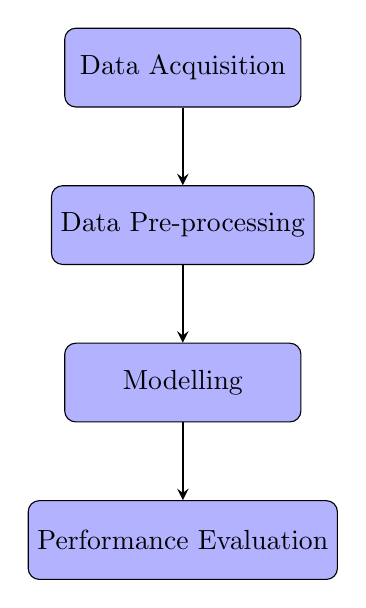
\begin{tikzpicture}[node distance=2cm]
        \node (start) [startstop] {Data Acquisition};
        \node (dc) [startstop, below of=start] {Data Pre-processing};
        \node (dpr) [startstop, below of=dc] {Modelling};
        \node (mtpe) [startstop, below of=dpr] {Performance Evaluation};
        \draw [arrow] (start) -- (dc);
        \draw [arrow] (dc) -- (dpr);
        \draw [arrow] (dpr) -- (mtpe);
    \end{tikzpicture}
    \caption{Traditional Machine Learning workflow}
    \label{fig:traditiona-ml-workflow}
\end{figure}

\subsection{Data Acquisition}

The first step in any machine learning project is acquiring the necessary data. This involves identifying and collecting datasets relevant to the problem at hand. The quality and quantity of the data directly impact the performance and generalization ability of the model. Data acquisition may involve obtaining datasets from public repositories, creating custom datasets, or integrating data from various sources.

\subsection{Data Pre-processing}

Once the data is collected, it undergoes pre-processing to make it suitable for training machine learning models. This stage involves cleaning the data to handle missing values, removing outliers, and addressing any inconsistencies. Additionally, feature engineering may be performed to extract relevant information and create new features. Data normalization or scaling may also be applied to ensure that all features contribute equally to the model.

\subsection{Modeling}

With pre-processed data, the next step is to select and train a machine learning model. This involves choosing an appropriate algorithm based on the nature of the problem (classification, regression, etc.) and the characteristics of the data. The selected model is then trained on a portion of the dataset, learning the patterns and relationships within the data. Hyperparameter tuning may be conducted to optimize the model's performance.

\subsection{Performance Evaluation}

The final stage of the traditional ML workflow is evaluating the model's performance on unseen data. This is typically done using a separate test dataset that the model has not encountered during training. Common evaluation metrics include accuracy, precision, recall, F1 score, and area under the receiver operating characteristic (ROC) curve. The goal is to assess how well the model generalizes to new, unseen instances and to identify areas for potential improvement.

\section{Bias}

Artificial Intelligence (AI) is undeniably a transformative force, poised to reshape multiple dimensions of the existence in profound ways. Its versatile applications extend far and wide, from refining and expediting decision-making processes to seamlessly automating mundane and repetitive tasks. In this ever-evolving landscape, AI systems are becoming increasingly integrated into daily experiences, orchestrating a paradigm shift in the way people interact with the world around them. 

However, amidst the excitement and optimism surrounding AI's potential, a growing concern resonates both within the AI community and society as a whole. This concern revolves around the pervasive issue of biases intricately woven into the very fabric of AI algorithms. 

These biases, often unintentional and subtle, can seep into AI systems through the data they are trained on and the methods employed to develop them. As AI systems learn from historical data, they may inadvertently inherit the prejudices and stereotypes present in those datasets. Consequently, these biases can manifest in various ways, perpetuating and amplifying societal inequalities. For example, in AI applications for hiring or lending, biases can result in unfair discrimination based on factors such as race or gender. In automated content recommendations, biases can reinforce echo chambers, limiting exposure to diverse perspectives and ideas. 

The consequences of these biases are far-reaching and profound. They not only undermine the ethical foundations of AI but can also erode trust in these technologies. As AI systems gain prominence in critical areas like healthcare, criminal justice, and education, the ramifications of bias become increasingly worrisome. 

Addressing bias in AI is a complex and ongoing challenge. It requires a multifaceted approach that encompasses not only improved data collection and curation but also transparency in AI decision-making processes. Researchers and engineers are working tirelessly to develop techniques for bias detection and mitigation. Additionally, there is a growing push for diverse representation in the AI development community to ensure that the creation of AI systems considers a wide array of perspectives. 

In conclusion, while the promise of AI is immense, the journey towards harnessing its potential responsibly and equitably is an imperative one. Moving forward in this AI-driven era, it is essential to remain vigilant in identifying and rectifying biases, ensuring that AI truly serves as a force for positive change in an always faster evolving world. \cite{10.1145/3308560.3317590}

\subsection{Understanding Bias in AI}

Bias in AI is a critical issue, signifying the presence of unjust and skewed representations or treatment of individuals or groups based on attributes such as race, gender, age, socioeconomic status, or other defining characteristics. These biases are deeply embedded in AI systems and can persist throughout their development and training processes. They arise from a variety of sources, including historical data imbalances, deeply ingrained societal prejudices, and imperfections in the algorithms themselves.

\subsection{Sources of Bias}

It's possible to establish 3 different sources of biases across several perspectives: historical, human and algorithmic perspective as well highlighted in \cref{fig:sources_of_bias}

\begin{figure}
    \centering
    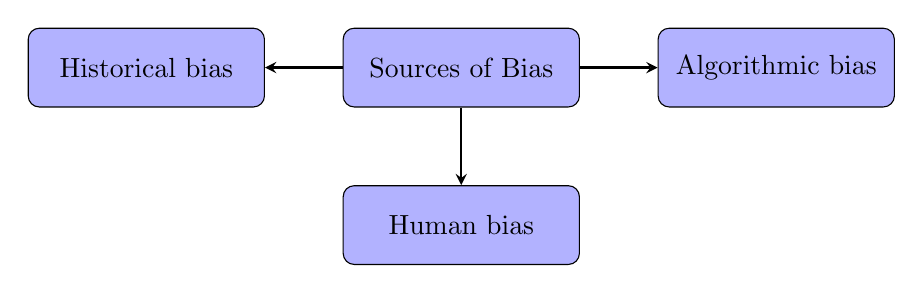
\begin{tikzpicture}[node distance=2cm]
        \node (start) [startstop] {Sources of Bias};
        \node (dc) [startstop, left of=start, xshift=-2cm] {Historical bias};
        \node (dpr) [startstop, below of=start] {Human bias};
        \node (mtpe) [startstop, right of=start, xshift=2cm] {Algorithmic bias};
        \draw [arrow] (start) -- (dc);
        \draw [arrow] (start) -- (dpr);
        \draw [arrow] (start) -- (mtpe);
    \end{tikzpicture}
    \caption{Sources of bias}
    \label{fig:sources_of_bias}
\end{figure}

\subsubsection{Historical bias} 

The issue of bias originating from historical data is a critical and intricate challenge that looms large in the landscape of machine learning. When machine learning models are trained on datasets culled from the annals of history, they inevitably inherit the biases and patterns encoded within that data. These historical biases, often a reflection of deeply ingrained societal prejudices and structural inequalities, can persist and intensify when the model is operationalized. \cite{10.1145/3308560.3317590}

Consider a scenario where historical data contains systemic biases against specific demographics, such as gender, race, or other socio-demographic attributes. The machine learning model, in its quest to optimize performance, dutifully replicates and perpetuates these biases in its predictions and decision-making processes. The consequence of this perpetuation is the perpetuation of historical injustices, potentially leading to the endorsement of discriminatory practices and the exacerbation of preexisting societal inequalities, significantly disadvantaging certain groups. 

Effectively addressing bias originating from historical data necessitates a multidimensional approach, coupled with proactive measures, as also showed in \cref{fig:h_b_addr}

\begin{enumerate}

    \item The first step involves diligent data preprocessing techniques aimed at the identification and subsequent mitigation of bias-laden elements within the dataset. These techniques span a spectrum from data re-sampling to re-weighting and data augmentation, designed to restore balance and fairness.

    \item Simultaneously, interventions in algorithmic fairness are introduced to the machine learning process. These interventions encompass a range of techniques, including re-weighting of training instances, the introduction of fairness constraints, and adversarial debiasing methods, all aimed at guiding the model toward making fair and equitable predictions. 

    \item Moreover, the journey toward equitable AI is an ongoing one, requiring constant vigilance. Continuous monitoring and adjustment of models, often in real-time, become imperative to ensure that fairness is upheld and biased outcomes are identified and rectified. 

\end{enumerate}

\begin{figure}
    \centering
    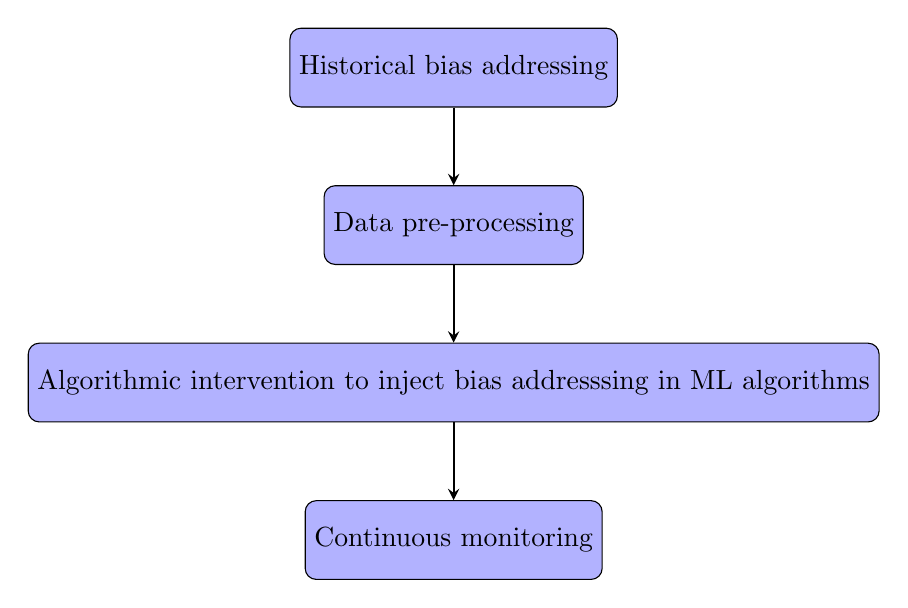
\begin{tikzpicture}[node distance=2cm]
        \node (start) [startstop] {Historical bias addressing};
        \node (dc) [startstop, below of=start] {Data pre-processing};
        \node (dpr) [startstop, below of=dc] {Algorithmic intervention to inject bias addresssing in ML algorithms};
        \node (mtpe) [startstop, below of=dpr] {Continuous monitoring};
        \draw [arrow] (start) -- (dc);
        \draw [arrow] (dc) -- (dpr);
        \draw [arrow] (dpr) -- (mtpe);
    \end{tikzpicture}
    \caption{Historical bias addressing}
    \label{fig:h_b_addr}
\end{figure}

Ultimately, the overarching goal is to foster a future where machine learning not only learns from historical data but actively works to transcend the bonds of bias. In this vision, AI systems operate as champions of fairness and social justice, contributing to the construction of a more equitable and just society where decisions and predictions are untainted by historical prejudices. This endeavor is not just a technical challenge but a moral imperative, driving the AI community to build a more equitable future for all.

\subsubsection{Human bias}

Bias introduced by human factors represents a pervasive and intricate challenge within the realm of machine learning. It is essential to understand that human bias, which can emanate from societal, cultural, or personal beliefs and attitudes, has the potential to inadvertently permeate the entire spectrum of the machine learning pipeline. This influence spans from the initial stages of data collection and annotation to the model training and decision-making processes. 

Human bias can manifest in multifarious ways, thereby complicating the quest for fair and unbiased machine learning models. These manifestations may include the biased selection of training data, subjectivity in annotations, or implicit prejudices that insidiously seep into the very fabric of algorithm design and evaluation. When humans are intricately involved in the decision-making processes or contribute to the development of algorithms, their biases, often unperceived, can become unintentionally embedded in the model. This results in a cascade of skewed predictions and the inadvertent reinforcement of preexisting societal inequalities. \cite{https://doi.org/10.1002/widm.1356} 

The recognition and mitigation of human bias represent an imperative for the development of equitable and just machine learning models. This mission encompasses several facets, as also showed in \cref{fig:hu_b_addr}

\begin{enumerate}

    \item First and foremost, it demands an elevated level of awareness within the machine learning community and society at large. Recognizing the potential pitfalls of human bias is a crucial step toward addressing them. 

    \item Promoting diversity and inclusion, both in the workforce and in the datasets used for model training, is instrumental in countering human bias. Diverse perspectives and a multiplicity of experiences contribute to a more comprehensive and unbiased understanding of the world. 

    \item Moreover, practical measures are implemented to detect and mitigate bias throughout the machine learning pipeline. This includes strategies ranging from fairness-aware machine learning algorithms to post-processing techniques that rectify biased predictions. 

    \item The journey toward mitigating human bias is continuous and iterative. Machine learning practitioners continually refine their algorithms to minimize the impact of human bias and ensure that their models contribute to a more equitable and unbiased society. 

\end{enumerate}

\begin{figure}
    \centering
    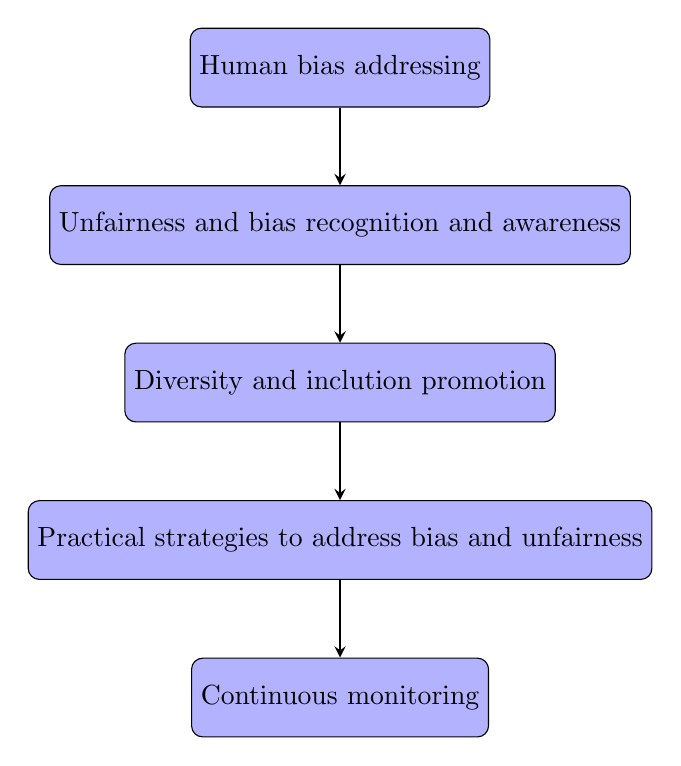
\begin{tikzpicture}[node distance=2cm]
        \node (start) [startstop] {Human bias addressing};
        \node (dc) [startstop, below of=start] {Unfairness and bias recognition and awareness};
        \node (dpr) [startstop, below of=dc] {Diversity and inclution promotion};
        \node (mtpe) [startstop, below of=dpr] {Practical strategies to address bias and unfairness};
        \node (cm) [startstop, below of=mtpe] {Continuous monitoring};
        \draw [arrow] (start) -- (dc);
        \draw [arrow] (dc) -- (dpr);
        \draw [arrow] (dpr) -- (mtpe);
        \draw [arrow] (mtpe) -- (cm);
    \end{tikzpicture}
    \caption{Human bias addressing}
    \label{fig:hu_b_addr}
\end{figure}

The ultimate goal is to harness the transformative potential of machine learning while eliminating the inadvertent perpetuation of human biases, thereby ushering in a more equitable and just era in technological advancement.

\subsubsection{Algorithmic bias}

Algorithmic bias, an intrinsic challenge in the domain of machine learning, underscores the presence of inherent biases that can manifest in the design, development, and deployment of machine learning algorithms. These biases, often unintended, can originate from a myriad of sources, encompassing factors such as biased training data, skewed feature selection, or implicit assumptions woven into the algorithm's development process. 

Algorithmic bias possesses the insidious potential to perpetuate and magnify preexisting societal prejudices and disparities, culminating in outcomes that are patently unfair and discriminatory. Consider the scenario in which a machine learning model is trained on historical data that inherently encapsulates societal biases. The model, in its endeavor to optimize predictive accuracy, inadvertently assimilates and reinforces these biases. The result is an algorithm that produces predictions and decisions that are tinged with bias, potentially aggravating societal inequalities and offering unequal treatment to specific groups. \cite{10.1145/2983270} 

The algorithmic bias mitigation requires several steps, as also showed in \cref{fig:alg_b_addr}:

\begin{enumerate}

    \item Addressing algorithmic bias is a pivotal imperative when striving to construct equitable and just AI systems. This undertaking encompasses a comprehensive scrutiny of the entire machine learning pipeline, from data collection to model development and deployment. It commences with the meticulous assessment and rectification of bias within training data, aiming to restore balance and fairness. 

    \item The integration of fairness-aware algorithms within the machine learning process is crucial. These algorithms are deliberately designed to recognize and rectify biases, offering a safeguard against discriminatory predictions and decisions.

    \item Transparency and fairness represent integral aspects of the decision-making process. The incorporation of these elements ensures that algorithms operate equitably, are devoid of bias, and actively promote fairness and equal treatment for all individuals, irrespective of their backgrounds. 

\end{enumerate}

\begin{figure}
    \centering
    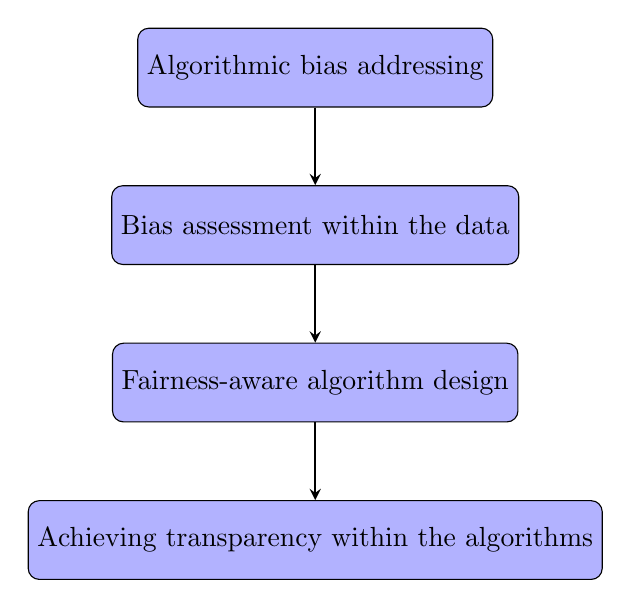
\begin{tikzpicture}[node distance=2cm]
        \node (start) [startstop] {Algorithmic bias addressing};
        \node (dc) [startstop, below of=start] {Bias assessment within the data};
        \node (dpr) [startstop, below of=dc] {Fairness-aware algorithm design};
        \node (mtpe) [startstop, below of=dpr] {Achieving transparency within the algorithms};
        \draw [arrow] (start) -- (dc);
        \draw [arrow] (dc) -- (dpr);
        \draw [arrow] (dpr) -- (mtpe);
    \end{tikzpicture}
    \caption{Algorithmic bias addressing}
    \label{fig:alg_b_addr}
\end{figure}

In essence, the mission of addressing algorithmic bias is pivotal for harnessing the true potential of AI systems. It involves forging a future where AI, far from perpetuating biases, serves as a champion of fairness and social justice, contributing to the construction of an equitable and just society in the digital age.

\subsection{Example of Bias in AI}

\subsubsection{Race and Gender Bias in Facial Recognition} 

Race and gender bias in facial recognition technology is a pressing and deeply concerning issue that underscores the ethical complexities tied to the development of AI. Facial recognition systems, often trained on large datasets, inadvertently perpetuate biases present in these datasets, particularly biases related to race and gender. The lack of diversity in training data, which is predominantly skewed towards certain demographics, results in algorithmic bias, where the system may struggle to accurately recognize individuals from underrepresented racial or gender groups. \cite{https://doi.org/10.5281/zenodo.4050457}

Studies have provided compelling evidence that these systems are often more accurate for individuals with lighter skin tones compared to those with darker skin tones, demonstrating a clear racial bias. Similarly, gender recognition algorithms may exhibit inaccuracies, especially for gender-nonconforming individuals, further exacerbating biases. 

The consequences of these biases are wide-ranging and profound. For instance, in law enforcement applications, the use of facial recognition may lead to the disproportionate targeting and misidentification of individuals from minority communities, potentially resulting in wrongful arrests and increased surveillance. In commercial contexts, biased facial recognition can significantly impact hiring processes, access to services, and overall societal fairness, with far-reaching implications for individuals and communities.


\subsubsection{Criminal Justice Bias}

Criminal justice bias is a deeply ingrained issue within the legal system that manifests through unequal treatment of individuals based on their race, socioeconomic status, gender, and other factors. The criminal justice system should ideally operate on principles of fairness, justice, and equality before the law. However, biases at various stages of the criminal justice process, from policing and arrest to trial and sentencing, often lead to discriminatory outcomes. \cite{doi:10.1080/10345329.2019.1658694} 

Racial bias is a significant concern, with people of color, especially Black individuals and communities, experiencing disproportionately higher rates of arrest, harsher sentencing, and a lack of trust in the system. Discriminatory practices such as racial profiling and racial disparities in sentencing contribute to this bias. Socioeconomic bias is another critical factor, where individuals from marginalized and low-income communities may face prejudice in the form of limited access to legal resources and unequal treatment within the legal process. \cite{9660177}  

Gender bias is prevalent, particularly against women and gender-diverse individuals. Women can face stereotypes and discriminatory attitudes that affect their treatment by law enforcement, the courts, and correctional facilities. Additionally, biases against LGBTQ+ individuals can result in unfair treatment and disparities in the criminal justice system. \cite{gebru2020race} 

Addressing criminal justice bias necessitates comprehensive reform. This includes implementing policies to combat racial and socioeconomic disparities, providing anti-bias training to law enforcement, encouraging diversity within the legal profession, and promoting transparency and accountability in the criminal justice process. Legislation, sentencing reform, community engagement, and the support of marginalized communities are also vital steps toward achieving a fair and impartial criminal justice system that upholds the principles of equity and justice for all.


\subsubsection{Recruitment Bias}

Recruitment bias is a critical issue within the hiring process, where unconscious or conscious prejudices and preconceived notions influence decision-making during candidate selection. It manifests in various forms, such as racial, gender, age, socio-economic, educational, or even appearance-based biases, and can significantly impact the composition of the workforce. \cite{mujtaba2019ethical} 

One of the most prevalent forms of recruitment bias is racial or ethnic bias. Hiring decisions can be influenced by stereotypes, leading to the underrepresentation of certain racial or ethnic groups in the workplace. Similarly, gender bias can result in disparities in hiring and promotion opportunities, favoring one gender over another. Age bias often affects older candidates who may be overlooked in favor of younger, perceived to be more 'tech-savvy' individuals. 

Educational and socio-economic biases can also seep into the hiring process, where candidates from prestigious institutions or privileged backgrounds may be given preferential treatment. Appearance-based biases, although highly unfortunate, can influence decisions, impacting individuals based on their physical attributes, such as weight, height, or even hairstyle. 

Addressing recruitment bias requires a multipronged approach. Firstly, raising awareness and providing training on unconscious bias is essential for hiring teams. Implementing structured and standardized interview processes, blind recruitment techniques (removing personally identifiable information), and diverse interview panels can help mitigate biases. Moreover, organizations should focus on promoting diversity and inclusion, fostering a culture that values different perspectives and backgrounds, and monitoring and analyzing recruitment data to identify patterns of bias. Striving for fairness and inclusivity in the hiring process not only leads to a more diverse workforce but also improves organizational innovation, creativity, and overall success.

\section{Fairness} 

The pursuit of fairness within AI systems represents a dynamic and indispensable area of focus within the ever-expanding realm of artificial intelligence. At its core, fairness underscores an ethical and moral imperative to ensure that AI technologies and algorithms treat all individuals with equitable respect, devoid of bias or discrimination. As AI increasingly penetrates diverse facets of society, from decision-making processes to job recruitment, lending, and law enforcement, the salience of fairness is unequivocal. 

The pursuit of fairness in AI is an all-encompassing endeavor, entailing an array of considerations that orbit around the ambition to eliminate bias predicated on attributes such as race, gender, age, ethnicity, and socio-economic status. Bias in AI manifests in multifarious ways, originating from the training data's inherent biases or the algorithms themselves. Fair AI systems, therefore, endeavor to minimize these biases, upholding the principles of impartiality and justice in the outcomes they produce. 

Addressing fairness within AI systems necessitates the employment of an assortment of techniques. This involves pre-processing data to ameliorate biases, the modification of algorithms to instill them with fairness-awareness, and post-processing methods to ensure that outcomes are equitable. Furthermore, transparency and explainability are pivotal features of AI models, facilitating a deeper understanding of potential biases and nurturing trust in the technology. 

Emphasizing the ethical dimension, the pursuit of fairness in AI systems transcends the confines of technical solutions. It necessitates the active involvement of stakeholders, the incorporation of diverse perspectives, and a steadfast commitment to adhering to guidelines and regulations that prioritize fairness and impartiality. 

In essence, the journey to achieve fairness in AI systems is an ongoing and multifaceted odyssey, demanding relentless research, interdisciplinary collaboration, and unwavering ethical vigilance. The ultimate objective is the creation of AI technologies that steadfastly uphold the principles of fairness, contributing to a more inclusive, just, and equitable society. The continued pursuit of fairness in AI is not just a technical endeavor but a moral imperative, shaping the future of technology and its impact on society.

\subsection{Fairness Techniques in AI}

\subsubsection{Pre-processing}

Pre-processing focuses on the pre-processing phase, an integral component of AI system development, is dedicated to the meticulous handling of data before it is utilized in the training of an AI model. This stage assumes paramount importance as it lays the foundation for equitable and unbiased AI systems, ensuring that the data used is both balanced and representative of the rich diversity inherent in the population. 

The objective of pre-processing is to rectify any imbalances, biases, or irregularities in the data, aiming to foster an environment where the AI model can operate without predisposition. The use of common pre-processing techniques is pivotal to this endeavor. These techniques encompass oversampling and undersampling, which seek to redress the imbalance in the distribution of data across various classes or groups. 

Additionally, pre-processing includes the meticulous removal of noise from the data. Noise, in this context, refers to extraneous or irrelevant information that could distort the model's learning process. The elimination of such noise serves to enhance the data's signal-to-noise ratio, improving the model's ability to discern meaningful patterns. 

Furthermore, the creation of balanced synthetic datasets is a valuable technique within the pre-processing repertoire. This involves the generation of new data points, often through the extrapolation of existing data, with the goal of augmenting the representation of underrepresented classes or groups. 

In summation, pre-processing is the cornerstone of equitable and unbiased AI system development. It encompasses a suite of techniques designed to foster balanced and representative data, enabling AI models to operate with impartiality and fairness, contributing to more equitable and unbiased outcomes. handling the initial data before it is used to train the AI model. This stage is crucial to ensure that the data is balanced and representative of the diversity in the population. Common pre-processing techniques include oversampling, undersampling, noise removal from the data, and creating balanced synthetic datasets.

\subsubsection{In-processing}

In-processing techniques represent a focused and interventionist approach that takes place directly during the model training phase. This method aims to instill fairness into the AI model at its core, ensuring equitable and unbiased outcomes. It is a precise and intricate strategy designed to mitigate bias and discrimination within the model's decision-making processes. 

One prominent in-processing technique involves the application of regularization methods. Regularization techniques are instrumental in penalizing the model when it demonstrates a discriminatory inclination, particularly with regard to certain sensitive features, such as gender or ethnic origin. By imposing penalties, the model is encouraged to refrain from exhibiting bias and to generate fair and impartial predictions. 

Another facet of in-processing techniques involves the alteration of cost functions. By modifying the cost functions, the model's training process is steered toward fairness. This modification ensures that the model pays a cost for making biased predictions, thereby incentivizing it to provide equitable treatment across different categories. 

In addition to regularization and cost function adjustments, in-processing techniques may encompass the manipulation of the model's predictions themselves. This manipulation can be guided by fairness constraints, ensuring that the model's outputs adhere to the principles of fairness and impartiality, especially concerning sensitive attributes. 

In summary, in-processing techniques serve as a focused and critical juncture in the quest for fairness within AI models. By intervening directly during the model training phase, these techniques work toward equitable and unbiased outcomes, promoting the development of AI technologies that contribute to a more fair and inclusive society.

\subsubsection{Post-processing}

Post-processing unfolds after the model has been meticulously trained and has generated predictions. This phase assumes the role of a corrective and fine-tuning mechanism, primarily focusing on adjustments and modifications to the model's predictions with the overarching objective of ensuring fairness and equity. 

One key facet of post-processing involves the application of realignments or adjustments to the model's predictions. These realignments are designed to rectify any unjustified disparities among demographic groups, ensuring that the model's outcomes are equitable and devoid of bias. This process may entail recalibrations or other transformative actions applied to the model's results to mitigate any latent biases that may have emerged during the training process. 

The successful implementation of post-processing techniques hinges on a profound understanding of the specific fairness challenges inherent in both the data and the models. This demands a nuanced comprehension of the intricacies of the data, including potential sources of bias and discrimination. Furthermore, it requires a comprehensive grasp of the model's inner workings, discerning where and why biases may have arisen. 

Ongoing evaluation represents an indispensable element of the post-processing phase. Continual assessments and audits are essential to ensure that AI models adhere to ethical standards and actively promote fairness. This continuous vigilance and adjustment are pivotal in fostering AI technologies that contribute to the construction of a more equitable and just society. 

In essence, post-processing represents the culmination of efforts to instill fairness within AI models, serving as the final safeguard against bias and discrimination in the model's predictions.


A comprehensive list of the several fairness techniques is showed in \cref{fig:fairness_techniques}

\begin{figure}
    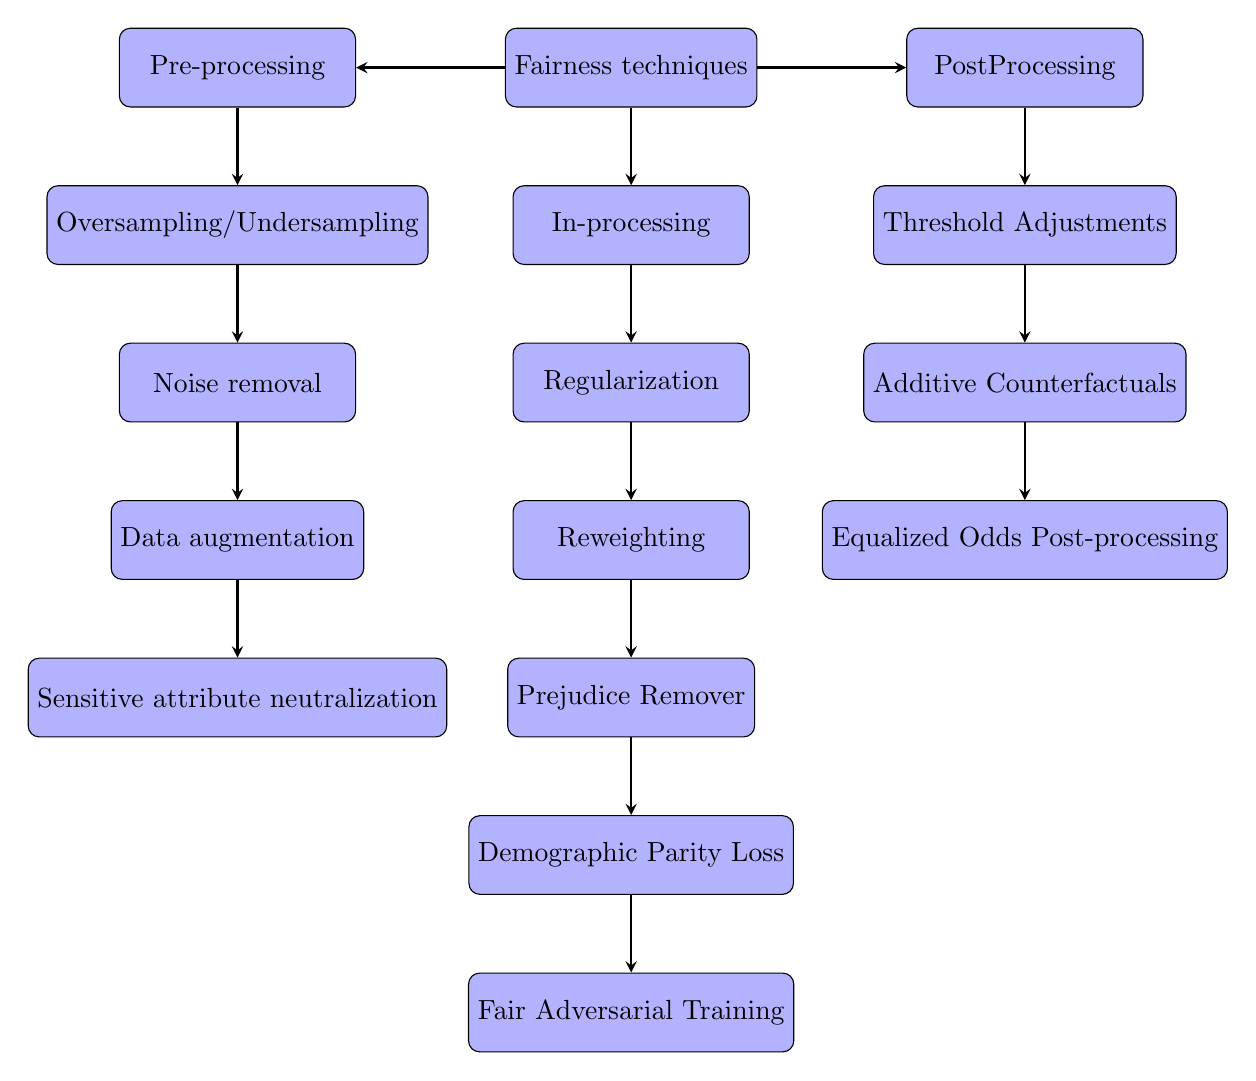
\begin{tikzpicture}[node distance=2cm]
        \node (start) [startstop] {Fairness techniques};
        \node (preproc) [startstop, left of=start, xshift=-3cm] {Pre-processing};
        \node (inproc) [startstop, below of=start] {In-processing};
        \node (postproc) [startstop, right of=start, xshift=3cm] {PostProcessing};
        \node (ou) [startstop, below of=preproc] {Oversampling/Undersampling};
        \node (nr) [startstop, below of=ou] {Noise removal};
        \node (da) [startstop, below of=nr] {Data augmentation};
        \node (sr) [startstop, below of=da] {Sensitive attribute neutralization};
        \node (re) [startstop, below of=inproc] {Regularization};
        \node (rew) [startstop, below of=re] {Reweighting};
        \node (pr) [startstop, below of=rew] {Prejudice Remover};
        \node (dp) [startstop, below of=pr] {Demographic Parity Loss};
        \node (fa) [startstop, below of=dp] {Fair Adversarial Training};
        \node (ta) [startstop, below of=postproc] {Threshold Adjustments};
        \node (ac) [startstop, below of=ta] {Additive Counterfactuals};
        \node (eo) [startstop, below of=ac] {Equalized Odds Post-processing};
        \draw [arrow] (start) -- (preproc);
        \draw [arrow] (start) -- (inproc);
        \draw [arrow] (start) -- (postproc);
        \draw [arrow] (preproc) -- (ou);
        \draw [arrow] (ou) -- (nr);
        \draw [arrow] (nr) -- (da);
        \draw [arrow] (da) -- (sr);
        \draw [arrow] (inproc) -- (re);
        \draw [arrow] (re) -- (rew);
        \draw [arrow] (rew) -- (pr);
        \draw [arrow] (pr) -- (dp);
        \draw [arrow] (dp) -- (fa);
        \draw [arrow] (postproc) -- (ta);
        \draw [arrow] (ta) -- (ac);
        \draw [arrow] (ac) -- (eo);
    \end{tikzpicture}
    \caption{Fairness addressing techniques}
    \label{fig:fairness_techniques}
\end{figure}


\subsection{Pre-processing Techniques for Addressing Fairness in AI}

Pre-processing techniques are applied before the training step, in orer to try to avoid bias and guarantee fairness to the data on which the ML models are trained. Several techniques can be emplyed in the pre-processing step:

\subsubsection{Oversampling and Undersampling}

Oversampling and undersampling are techniques used to address class imbalance, where one class significantly outnumbers the others in a dataset. In the context of fairness, these techniques are employed to ensure that the AI model is not biased towards the majority class and that the predictions are fair and equitable for all classes, particularly when sensitive attributes like race, gender, or ethnicity are involved. \cite{9442706}

\begin{enumerate}

    \item \emph{Oversampling}

    \begin{itemize}

        \item \emph{Definition:} Oversampling involves increasing the number of instances in the minority class by generating synthetic samples or replicating existing ones.
        
        \item \emph{Fairness Context:} Oversampling aims to boost the representation of underrepresented groups, promoting fairness and equal consideration of all groups. It prevents the model from exhibiting bias towards the majority group.
    
    \end{itemize}

    \item \emph{Undersampling}

    \begin{itemize}

        \item \emph{Definition:} Undersampling involves reducing the number of instances in the majority class by removing samples, ideally in a strategic and unbiased manner.
        
        \item \emph{Fairness Context:} Undersampling can be employed to level the playing field by reducing the dominance of the majority group. This ensures that the model's predictions are not disproportionately influenced by the majority group, promoting fairness in the model's outcomes.
    
    \end{itemize}

\end{enumerate}

\subsubsection{Noise Removal}

Noise removal in the context of fairness typically refers to the process of identifying and mitigating the effects of noisy or incorrect data points that may introduce biases or distortions in the data used to train or evaluate machine learning models. In fairness considerations, noise removal plays a crucial role in ensuring that the AI system's predictions and decisions are as accurate and unbiased as possible, particularly when sensitive attributes like race, gender, or ethnicity are involved. \cite{NEURIPS2019_8d5e957f}

\subsubsection{Data Augmentation}

Data augmentation is a technique often used in machine learning and data preprocessing to artificially increase the size and diversity of a training dataset by generating new data points based on the existing ones. In the context of fairness, data augmentation can play a crucial role in addressing imbalances and biases in the data, particularly when sensitive attributes are involved. Here's how data augmentation can be applied in the context of fairness:

\begin{enumerate}

    \item \emph{Generating Additional Data for Underrepresented Groups}
    
    \begin{itemize}

        \item In scenarios where certain groups or classes are underrepresented in the training data, data augmentation techniques can be used to create additional examples for those groups. \cite{sharma2020data}
    
    \end{itemize}
    
    \item \emph{Balancing Class or Group Representation}
    
    \begin{itemize}
        
        \item Data augmentation can be employed to balance class or group representation in the training data. By creating synthetic data points for underrepresented groups, it helps ensure that the model is not biased towards majority groups.
    
    \end{itemize}
    
    \item \emph{Feature Engineering for Fairness}
    
    \begin{itemize}
        
        \item Data augmentation can also involve feature engineering that considers sensitive attributes. For example, it can create new features that better capture the nuances and characteristics of underrepresented groups. \cite{10.14778/3461535.3463474}
    
    \end{itemize}
    
    \item \emph{Fair Data Augmentation}
    
    \begin{itemize}
    
        \item In the fairness context, it's important to ensure that data augmentation techniques do not introduce additional biases. Care should be taken to create synthetic data that aligns with the fairness and equity goals of the AI system. \cite{10.1145/3531146.3534644}
    
    \end{itemize}

\end{enumerate}

\subsubsection{Bias Mitigation Algorithms}

Bias mitigation in the context of fairness refers to the process of identifying, reducing, or eliminating biases within machine learning models and algorithms, particularly those that could lead to unfair or discriminatory outcomes, often associated with sensitive attributes like race, gender, age, or ethnicity. The goal of bias mitigation is to ensure that AI systems provide equitable and unbiased predictions and decisions for all individuals or groups.

\subsubsection{Sensitive Attribute Removal or Neutralization}

In some cases, sensitive attributes (e.g., race, gender) can be removed from the dataset or transformed into more neutral representations. This prevents the model from relying on these attributes to make predictions, promoting fairness. \cite{NEURIPS2021_64ff7983}

These pre-processing techniques are essential steps in the AI development pipeline to ensure that the subsequent models are fair, unbiased, and capable of providing equitable outcomes across various demographic categories.

\subsection{In-processing Techniques for Addressing Fairness in AI}

In-processing techniques aim to mitigate fairness issues directly during the model training phase, influencing the learning process to ensure fairness in model predictions. These approaches target bias reduction and fairness promotion within the model's decision-making process. Several techniques can be employed during model training to achieve fairness:

\subsubsection{Regularization}

Regularization  aims to address and mitigate potential biases within models, particularly when sensitive attributes like race, gender, or ethnicity are involved. Regularization techniques work by adding constraints or penalties to the model's training process to reduce the impact of sensitive attributes on predictions and ensure that fairness is maintained. \cite{6137441}

\subsubsection{Reweighting Training Samples}

Reweighting training samples is a technique used to address bias and promote fairness in machine learning models, particularly when sensitive attributes are involved. This approach involves assigning different weights to training samples to influence the learning process of the model in a way that mitigates bias and ensures that predictions are more equitable. \cite{10.1145/3178876.3186133}

\subsubsection{Prejudice Remover Regularizer}

The Prejudice Remover Regularizer is a technique used to mitigate bias and promote equitable outcomes in machine learning models. It's a form of regularization that aims to reduce discrimination by encouraging the model to make predictions that are less influenced by sensitive attributes such as race, gender, or ethnicity. \cite{10.1007/978-3-642-33486-3_3}

\subsubsection{Demographic Parity Loss}

The Demographic Parity Loss is a fairness metric and regularization technique used to promote fairness and reduce bias, particularly with regard to sensitive attributes like race, gender, or ethnicity. It is designed to ensure that the predictions made by a model are distributed equally or fairly across different demographic groups. \cite{jiang2022generalized}

\subsubsection{Fair Adversarial Training}

Fair adversarial training is a technique used in the context of fairness to reduce bias and discrimination in machine learning models, particularly when sensitive attributes like race, gender, or ethnicity are involved. This approach incorporates adversarial networks into the training process to promote fairness and equitable outcomes. \cite{pmlr-v139-xu21b}

These in-processing techniques are vital tools in promoting fairness within AI models. Integrating them appropriately during model training can significantly contribute to reducing biases and achieving equitable outcomes across various demographic categories.

\subsection{Post-processing Techniques for Addressing Fairness in AI}

Post-processing techniques are applied after the model has been trained and predictions have been generated. Their purpose is to rectify any biases or disparities in the model's outputs and ensure fairness in the final outcomes. Several techniques can be employed during post-processing to promote fairness:

\subsubsection{Threshold Adjustments}

Threshold adjustment is a technique used to promote equity and reduce bias in machine learning models, especially in scenarios where sensitive attributes like race, gender, or age play a significant role. It involves modifying the decision threshold that determines whether a model's output is classified as a positive or negative prediction. This adjustment aims to balance the rates of false positives and false negatives across different demographic or group categories, ensuring that all groups are treated more fairly. \cite{10.1145/3447548.3467251}

\subsubsection{Additive Counterfactuals}

Additive counterfactual explanations in the context of fairness refer to a method used to assess and promote fairness in machine learning models. Counterfactual explanations are designed to provide insights into the impact of sensitive attributes on model predictions and help identify potential bias or discrimination. The additive aspect suggests that changes are made to the original input to create counterfactual scenarios, allowing for a better understanding of the fairness implications. \cite{NIPS2017_a486cd07}

\subsubsection{Equalized Odds Post-processing}

Equalized Odds Post-processing is a technique used to mitigate bias and promote equal treatment in machine learning models, particularly in scenarios involving binary classification tasks. This technique is applied after a model has made predictions and aims to adjust those predictions to ensure that equal error rates are achieved across different demographic or group categories. \cite{10.1145/3442188.3445902}

These post-processing techniques are crucial in rectifying biases and promoting fairness in AI models. Utilizing them effectively can lead to more equitable outcomes and decisions across various demographic categories.

\section{Fair-by-Design}

Fair-by-design methods represent a proactive approach to addressing bias and promoting fairness in machine learning and artificial intelligence systems from their inception. These methods aim to embed fairness considerations into the design and development of algorithms and models to prevent bias from emerging in the first place. 

There are several key aspect to consider during the development of a Fair-by-Design method:

\begin{itemize}

    \item A careful curation and preprocessing of training data to mitigate biases that might be present. For instance, techniques for re-sampling, re-weighting, and data augmentation can be employed to balance underrepresented groups in the data.

    \item It's required the modification of algorithms to incorporate fairness-awareness. This can be achieved through the introduction of fairness constraints during the training process or through adversarial debiasing techniques.

    \item Post-processing methods are often utilized to ensure that the outcomes of machine learning models are equitable. These methods can include adjusting the model's predictions to reduce disparities between different groups.

\end{itemize}

The ultimate goal of fair-by-design methods is to create AI systems that, from their very conception, are inherently fair and unbiased. By considering fairness as a fundamental design principle, it's possible to work towards eliminating discriminatory effects in AI systems, contributing to a more equitable and just technological landscape. 

\section{Fairness notions}
\label{section:fairness_notions}

Fairness notions serve as the foundational pillars that define the ethical considerations and objectives guiding the development of fair AI systems. These notions articulate specific principles for mitigating bias and promoting fairness, each with its unique characteristics and mathematical underpinnings.

\subsection{Demographic Parity}

Demographic Parity represents a fundamental fairness notion that addresses the equal representation of protected groups across different outcomes. In a binary classification context, it can be expressed as:

\[ P(\hat{Y} = 1 | A = a) = P(\hat{Y} = 1), \]

where \( \hat{Y} \) denotes the predicted outcome, \( A \) is the protected attribute, and \( a \) signifies a specific value of the protected attribute. The goal of Demographic Parity is to ensure that the distribution of positive outcomes is consistent across various demographic groups. While conceptually straightforward, Demographic Parity may overlook nuances in individual experiences and predictive accuracy.

\subsection{Equalized Odds}

Equalized Odds is a fairness notion that focuses on balancing the true positive and false positive rates across protected groups. Mathematically, it can be formalized as:

\[ P(\hat{Y} = 1 | A = a, Y = y) = P(\hat{Y} = 1 | Y = y), \]

where \( Y \) represents the true outcome. Equalized Odds strives to rectify disparities in prediction accuracy between protected groups, ensuring that both favorable and unfavorable outcomes are predicted with similar precision. This notion addresses concerns related to disparate error rates and aims to provide equal predictive performance for different demographic groups.

\subsection{Individual Fairness}

Individual Fairness introduces a nuanced dimension by emphasizing the fair treatment of similar individuals, irrespective of their protected attributes. While challenging to formalize precisely, it can be understood as:

\[ d(x, x') \leq \epsilon \Rightarrow |P(\hat{Y} = 1 | X = x, A = a) - P(\hat{Y} = 1 | X = x', A = a)| \leq \delta, \]

where \( d(x, x') \) measures the similarity between instances \( x \) and \( x' \), and \( \epsilon \) and \( \delta \) are predefined thresholds. Individual Fairness recognizes the unique characteristics of each instance and aims to ensure comparable treatment for similar individuals.

\subsection{Group Fairness}

Group Fairness extends fairness considerations to demographic groups, focusing on statistical parity in predicted outcomes. Formally, it can be expressed as:

\[ P(\hat{Y} = 1 | A = a) = P(\hat{Y} = 1 | A = a'), \]

where \( a \) and \( a' \) denote different values of the protected attribute. Group Fairness advocates for equitable treatment at the collective level, ensuring parity in the overall distribution of predicted outcomes among various demographic groups.

\section{Fairness metrics}
\label{section:metrics}

Fairness metrics play a crucial role in evaluating the performance of AI systems and ensuring equitable outcomes for diverse groups. These metrics provide quantitative measures to assess and mitigate bias within machine learning models. In this section, it will explored the general concept of fairness metrics and delve into three specific metrics: disparate impact, equalized odds, and demographic parity.

\subsection{General Overview}

Fairness metrics are quantitative tools designed to assess the impact of AI systems on different demographic groups. They help identify and address biases in model predictions, ensuring that the system does not disproportionately favor or disadvantage specific groups based on protected attributes such as race, gender, or age.

Common fairness metrics include disparate impact, equalized odds, demographic parity, and many others. These metrics are instrumental in evaluating the fairness and ethical implications of AI models, particularly in applications like hiring, lending, and education.

\subsection{Disparate Impact}

\emph{Definition:}

Disparate impact measures the ratio of favorable outcomes for different demographic groups. It highlights situations where a particular group experiences a disproportionately adverse impact compared to others.

\emph{Calculation:}
\[ DI = \frac{Pr(Y = 1|A=a)}{Pr(Y = 1|A=b)} \]

Where:
\begin{itemize}
    \item \( Y \) is the predicted outcome,
    \item \( A \) is the sensitive attribute (e.g., gender, race),
    \item \( a \) and \( b \) represent different values of the sensitive attribute.
\end{itemize}

\emph{Interpretation:}

A disparate impact value close to 1 indicates fairness, while values significantly deviating from 1 suggest potential bias.

\subsection{Equalized Odds}

\emph{Definition:}

Equalized odds ensures that the true positive rate and false positive rate are similar across different demographic groups. This metric focuses on achieving parity in both the benefits and errors of the model for different groups.

\emph{Calculation:}

\[ \text{True Positive Rate (TPR)} = \frac{Pr(\hat{Y} = 1|Y = 1, A = a)}{Pr(Y = 1|A = a)} \]
\[ \text{False Positive Rate (FPR)} = \frac{Pr(\hat{Y} = 1|Y = 0, A = a)}{Pr(Y = 0|A = a)} \]

\emph{Interpretation:}

Equalized odds is achieved when the TPR and FPR are approximately equal across all demographic groups.

\subsection{Demographic Parity}

\emph{Definition:}

Demographic parity requires that the proportion of positive outcomes is the same for all demographic groups, regardless of the sensitive attribute.

\emph{Calculation:}

\[ DP = Pr(\hat{Y} = 1|A = a) - Pr(\hat{Y} = 1|A = b) \]

\emph{Interpretation:}

A value close to 0 indicates fairness, suggesting that the model's predictions are not influenced by the sensitive attribute.

\section{Fairlearn Library}
\label{section:fairlearn}

Fairlearn is a powerful and versatile open-source Python library developed to address fairness concerns in machine learning models. Recognizing the importance of mitigating biases and ensuring equitable outcomes, Fairlearn provides a comprehensive set of tools, algorithms, and metrics designed to facilitate fairness-aware model development and evaluation.

\subsection{Key Features of Fairlearn}

Fairlearn offers a range of key features that empower researchers and practitioners to assess and enhance the fairness of their machine learning models:

\subsubsection{Fairness Metrics}

The library includes a diverse set of fairness metrics that enable quantitative assessment of bias and disparity in model predictions. Metrics such as disparate impact, equalized odds, and demographic parity provide insights into the impact of model decisions on different demographic groups.

\subsubsection{Algorithms}

Fairlearn incorporates fairness algorithms tailored for pre-processing, in-processing, and post-processing stages of the machine learning pipeline. These algorithms aim to mitigate biases and promote fairness in model predictions, offering flexibility for users to choose and integrate the most suitable techniques for their specific applications.

In conclusion, fairness in AI is not just an ethical necessity but a fundamental requirement for fostering trust and ensuring the responsible and equitable deployment of AI systems. Moving into the evolving landscape of AI, the collective efforts must prioritize fairness to harness the true potential of AI for the greater good.
%Write background here.

%This section is likely to contain a lot of citations.
%
%For instance in \cite{AnzengruberSocInfo2013} the authors propose a novel means for tackling with the problem of preventing bad things from happening.


%----------------------------------------------------------------------------------------
\chapter{Contribution} % possible chapter for Projects
\label{chap:contribution}

\section{Introduction to the Fair-by-Design Workflow}
\label{section:workflow-introduction}

In recent years, heightened scrutiny of the ethical implications associated with artificial intelligence (AI) and machine learning (ML) systems has arisen in response to the escalating influence of these technologies, particularly in domains where consequential decisions profoundly impact individuals' lives. The evolving landscape of AI ethics necessitates a conscientious examination of the ethical dimensions embedded in the development and deployment of these systems.

Amid this multifaceted ethical discourse, the imperative of integrating fairness into the fabric of AI design has emerged as a paramount consideration. The principle of fairness, when applied as a foundational element in the design process, underscores the need for AI systems to produce outcomes that are not only accurate and efficient but also just and equitable. Achieving fairness in AI development demands a comprehensive and deliberate approach, one that transcends mere post hoc considerations by embedding fairness principles from the very inception of the design process.

The conceptual framework of a Fair-by-Design (FBD) workflow encapsulates a meticulous set of principles and procedural steps, each strategically devised to ensure the attainment of equitable and unbiased outcomes throughout the entire lifecycle of an AI system. This includes not only the initial design and development phases but also extends to the implementation, deployment, and ongoing monitoring stages. The iterative nature of this workflow acknowledges the dynamic interplay between ethical considerations and technological advancements, emphasizing the continuous reassessment and refinement of fairness strategies.

By adopting a Fair-by-Design approach, stakeholders in AI development, ranging from researchers and engineers to policymakers and end-users, commit to a shared responsibility for cultivating a technological landscape where the ethical imperatives of fairness and equity are not afterthoughts but integral components steering the trajectory of AI systems towards societal benefit and justice. In essence, the pursuit of ethical AI underscores not only the advancement of technological capabilities but also the conscientious stewardship of these capabilities to ensure they align with ethical norms and societal values.


\subsection{Principles of Fair-by-Design Workflow}
\label{subsection:workflow-principles}

\begin{enumerate}[label=\arabic*.]
    \item \emph{Proactive Fairness Integration:}
    
    \begin{itemize}
       
        \item The cornerstone of the Fair-by-Design workflow lies in the proactive embedding of fairness considerations at the genesis of the design process, diverging from conventional practices where fairness is often retroactively addressed after system implementation.
        
        \item This proactive approach marks a transformative shift in the landscape of algorithmic development, underscoring the ethical imperative of forethought in anticipating and mitigating biases.
        
        \item Seamless integration of fairness into the initial design stages aims to forestall the emergence of discriminatory outcomes, establishing a bedrock rooted in equitable principles.
        
        \item Beyond its alignment with ethical standards, this proactive integration streamlines the developmental trajectory, fostering a more responsible and inclusive machine learning environment.
       
        \item This meticulous attention to fairness from the inception reflects a commitment to ethical AI practices that transcend mere compliance, embodying a conscientious endeavor to uphold societal values and ensure the equitable treatment of diverse individuals impacted by AI systems.
   
    \end{itemize}

    \item \emph{Transparency and Explainability:}
    
    \begin{itemize}
        
        \item The Fair-by-Design workflow places a premium on transparent documentation of design decisions and algorithmic choices, considering it a fundamental pillar of its ethical framework.
       
        \item Meticulous documentation serves as a deliberate and strategic endeavor to enhance accountability and foster trust among stakeholders.
       
        \item Each decision, ranging from the selection of specific algorithms to the fine-tuning of parameters, is comprehensively recorded, creating a clear and accessible trail of the workflow's development trajectory.
       
        \item This commitment to transparency is deeply rooted in the conviction that open communication of design rationales and choices cultivates a sense of reliability and confidence among stakeholders.
       
        \item By actively promoting transparency, the Fair-by-Design workflow contributes to the creation of a trustworthy and ethically grounded landscape for the deployment of machine learning systems.
       
        \item The deliberate and open documentation not only satisfies ethical considerations but also facilitates a more robust understanding of the system's inner workings, empowering stakeholders to engage meaningfully in the ongoing dialogue surrounding the ethical dimensions of AI technologies.
    
    \end{itemize}

    \item \emph{User-Centered Approach:}
   
    \begin{itemize}
      
        \item Within the Fair-by-Design workflow, the integration of diverse perspectives transcends a passive consideration; it stands as a proactive and integral aspect of the design process.
      
        \item The voices and perspectives of end-users and relevant stakeholders are not only actively sought but thoughtfully incorporated from the early stages of system design.
      
        \item This inclusive approach is designed to ensure that the developed system is finely tuned to the diverse needs, expectations, and concerns of its user base.
     
        \item Stakeholder engagement takes on various forms, ranging from surveys and interviews to collaborative workshops.
      
        \item These mechanisms allow for a comprehensive understanding of the social, cultural, and ethical dimensions that may influence system usage.
       
        \item Actively involving end-users and stakeholders in the design process serves a dual purpose: promoting inclusivity and enhancing the likelihood of developing a system that genuinely serves and respects the interests of its users.
       
        \item This user-centered approach is not merely a procedural step but a foundational commitment to creating AI systems that align with the values and requirements of the communities they impact.
    
    \end{itemize}

    \item \emph{Continuous Monitoring and Iterative Development:}
    
    \begin{itemize}
     
        \item Beyond the initial implementation, the Fair-by-Design system adopts a vigilant and continuous monitoring regimen, constituting a pivotal component of its iterative workflow.
     
        \item This meticulous monitoring process is crafted to detect and address emerging fairness issues that may manifest during system operation.
     
        \item Leveraging advanced monitoring tools and techniques, the workflow ensures that the system's performance is regularly assessed in real-world scenarios.
      
        \item This proactive approach enables the timely identification of potential biases or disparities, allowing for the swift implementation of corrective measures.
     
        \item The iterative nature of the workflow is a testament to its adaptability, facilitating ongoing refinements to ensure that the system evolves in response to changing dynamics and user experiences.
     
        \item This commitment to continuous monitoring and improvement underscores the Fair-by-Design philosophy: an emphasis not only on achieving fairness at a single point in time but on actively maintaining and enhancing fairness throughout the system's entire lifecycle.
      
        \item By embracing a dynamic and iterative model, the Fair-by-Design workflow remains resilient, ensuring that it remains responsive to the evolving landscape of ethical considerations and technological advancements in artificial intelligence.
   
    \end{itemize}

\end{enumerate}

\section{Steps to Implement a Fair-by-Design Workflow}
\label{section:steps}

\begin{enumerate}

    \item \emph{Objective Definition:} Clearly articulate the objectives of the system or process being designed, emphasizing the importance of fairness.

    \item \emph{Data Collection:} Determine the types of data needed for the application, establish ethical data collection protocols.

    \item \emph{Data pre-processing:} Prepare the data for the fairness algorithm, through data cleaning and featyre engineering
    
    \item \emph{Algorithmic Design and Definitions:} Define and implement fairness-enhancing algorithms across pre-processing, in-processing, and post-processing stages. Provide detailed definitions and explanations for each algorithm.

    \item \emph{Model training and evaluation:} Define the training step, performs the training tuning certain parameters and provides an evaluation of the performances of the models based on accuracy and fairness metrics.

\end{enumerate}


\begin{figure}[H]
    \centering
    \includegraphics[width=.3\textwidth, height=.8\textwidth]{workflow-steps.png}
    \label{fig:steps}
    \caption{Fair-by-Design steps}
\end{figure}
    

\subsection{Objective Definition}
\label{subsection:objective}

The first critical step in the Fair-by-Design workflow involves a precise definition of the objectives, laying the groundwork for subsequent fairness considerations. This stage encompasses the identification of the goal of the study, the identification of protected attributes, the selection of fairness notions, and the choice of an appropriate fairness metric.

\subsubsection{Goal of the study}

The first target in the Fair-by-Design workflow is related to the identification of the goal of the whole study. It's fundamental to be able to understand whether the study requires a classification approach or a regression.


\subsubsection{Protected Attributes}

Protected attributes refer to the characteristics of individuals or groups that are explicitly considered to prevent discrimination and bias. The criteria for choosing specific protected attributes must be well-defined to ensure the relevance of fairness considerations. This may involve:

\begin{itemize}

    \item Conducting a comprehensive literature review to identify historically disadvantaged or underrepresented groups.
    
    \item Collaborating with domain experts, ethicists, and stakeholders to determine attributes with potential societal impact.
    
    \item Assessing the legal and ethical implications of including or excluding certain attributes within the specific context of the AI application.

\end{itemize}

The selected protected attributes form the basis for subsequent fairness evaluations and interventions.

\subsubsection{Fairness Notions}

Fairness notions represent the abstract principles guiding the desired equitable behavior within the AI system. The choice of fairness notions is a pivotal decision, influencing subsequent stages of the workflow. Common fairness notions, as explained in detail in \cref{section:fairness_notions}, include:

\begin{itemize}
  
    \item \textbf{Demographic Parity:} Ensuring equal representation of protected groups across different outcomes.
  
    \item \textbf{Equalized Odds:} Balancing the true positive and false positive rates across protected groups.
  
    \item \textbf{Individual Fairness:} Treating similar individuals similarly, regardless of their protected attributes.
   
    \item \textbf{Group Fairness:} Ensuring fair treatment for entire groups, typically based on statistical measures.

\end{itemize}

The selection of a fairness notion should align with the specific goals of the AI application, ethical considerations, and legal requirements.

\subsubsection{Fairness Metric}

A fairness metric quantifies the level of fairness achieved by the AI system with respect to the chosen fairness notion. The choice of a fairness metric depends on the specific fairness notion and the underlying characteristics of the data. Common fairness metrics include:

\begin{itemize}
   
    \item \textbf{Disparate Impact:} Measures the ratio of favorable outcomes between protected and unprotected groups.
   
    \item \textbf{Equalized Odds Difference:} Quantifies the disparity in error rates between protected groups.
   
    \item \textbf{Theil Index:} Evaluates the distribution of outcomes across different demographic groups.
   
    \item \textbf{Statistical Parity Difference:} Measures the difference in favorable outcomes between protected and unprotected groups.

\end{itemize}

\subsubsection{Fairness Notions and Metric Alignment}
\label{subsub:alignment}

The alignment between fairness notions and fairness metrics is a critical aspect of the Fair-by-Design workflow, as it establishes a systematic and measurable framework for evaluating fairness. The following considerations guide the selection process:

\paragraph{Demographic Parity:}

For the fairness notion of Demographic Parity, the primary concern is ensuring equal representation of protected groups across different outcomes. This notion is often aligned with the fairness metric known as \textbf{Disparate Impact}, which quantifies the ratio of favorable outcomes between protected and unprotected groups. Specifically, the Disparate Impact metric is calculated as:

\[
\text{Disparate Impact} = \frac{\text{Favorable Outcome Rate for Protected Group}}{\text{Favorable Outcome Rate for Unprotected Group}}
\]

A Disparate Impact value close to 1 indicates a balanced representation, while values significantly deviating from 1 may suggest unfairness.

\paragraph{Equalized Odds:}

The Equalized Odds fairness notion aims to balance the true positive and false positive rates across protected groups. This aligns with the \textbf{Equalized Odds Difference} fairness metric, which quantifies the disparity in error rates between protected groups. The Equalized Odds Difference is computed as:

\[
\text{Equalized Odds Difference} = \text{True Positive Rate}_{\text{Protected}} - \text{True Positive Rate}_{\text{Unprotected}}
\]

A value of 0 indicates perfect balance, with positive or negative values signifying imbalances in the error rates.

\paragraph{Individual Fairness:}

Individual Fairness focuses on treating similar individuals similarly, regardless of their protected attributes. This notion is inherently challenging to quantify, but proxy metrics such as \textbf{Theil Index} may be employed. The Theil Index evaluates the distribution of outcomes across different demographic groups and is given by:

\[
\text{Theil Index} = \sum \left( \frac{X_{i}}{\mu} \ln \frac{X_{i}}{\mu} \right)
\]

where \(X_{i}\) represents the outcome distribution for a specific group, and \(\mu\) is the overall average outcome. A lower Theil Index indicates a more equitable distribution.

\paragraph{Group Fairness:}

Group Fairness ensures fair treatment for entire groups, typically based on statistical measures. The \textbf{Statistical Parity Difference} is a common metric aligned with this notion. It measures the difference in favorable outcomes between protected and unprotected groups and is computed as:

\[
\text{Statistical Parity Difference} = \text{Favorable Outcome Rate}_{\text{Prot}} - \text{Favorable Outcome Rate}_{\text{Unprot}}
\]

A value of 0 suggests parity, while positive or negative values indicate disparities.

These alighnments are well-represented in the following table


\begin{tabular}{|c|c|}
    \hline
    \textbf{Fairness notion} & \textbf{Fairness metric} \\
    \hline
    Demographic Parity & Disparate Impact \\
    \hline
    Equalized Odds & Equalized Odds Difference \\
    \hline
    Individual Fairness & Theil Index \\
    \hline
    Group Fairness & Demographic Parity Difference \\
    \hline
\end{tabular}

\subsubsection{Choosing Fairness Metrics Given Notions or Vice Versa}

Choosing a fairness metric given a fairness notion, or vice versa, requires a nuanced understanding of the specific fairness goals and the characteristics of the data. Here's a step-by-step guide:

\paragraph{Given a Fairness Notion:}

\begin{enumerate}
 
    \item \textbf{Define Fairness Goals:} Clearly articulate the fairness goals, considering the desired equitable outcomes for protected groups.
 
    \item \textbf{Identify Relevant Fairness Notion:} Select the fairness notion that aligns most closely with the defined fairness goals (e.g., Demographic Parity, Equalized Odds, Individual Fairness, or Group Fairness).
 
    \item \textbf{Choose Aligned Fairness Metric:} Based on the selected fairness notion, choose the fairness metric that provides a quantitative measure of the specified fairness goals (e.g., Disparate Impact, Equalized Odds Difference, Theil Index, or Statistical Parity Difference).

\end{enumerate}

\paragraph{Given a Fairness Metric:}

\begin{enumerate}

    \item \textbf{Understand Fairness Metric:} Gain a deep understanding of the chosen fairness metric, considering its strengths, limitations, and relevance to specific fairness goals.

    \item \textbf{Determine Fairness Notion Alignment:} Identify the fairness notion that aligns with the underlying principles of the chosen fairness metric (e.g., Disparate Impact aligns with Demographic Parity).
 
    \item \textbf{Ensure Consistency:} Confirm that the selected fairness metric is consistent with the broader fairness goals and ethical considerations of the AI application.

\end{enumerate}

This decisional process is well-represented in the following image:

\begin{figure}[h]
    \centering
    \includegraphics[width=.9\textwidth, height=1.3\textwidth]{notion-metric.png}
    \label{fig:choice}
    \caption{Fairness Notion and Metric choice}
\end{figure}

This meticulous alignment process ensures that the chosen fairness metrics quantitatively capture the intended fairness notions, providing a meaningful and interpretable basis for evaluating and comparing fairness across different models and interventions within the Fair-by-Design workflow.

In summary, the objective definition stage of the Fair-by-Design workflow involves a meticulous and well-informed selection of protected attributes, fairness notions, and fairness metrics. This precision ensures the subsequent stages of the workflow are grounded in a robust foundation for addressing bias and promoting fairness in AI systems.

\subsection{Data Collection}
\label{subsection:data_collection}

The data collection stage is fundamental for the Fair-by-Design workflow. It involves systematically gathering data to train machine learning models, coupled with a detailed study of the dataset's statistical properties, with a specific focus on protected attributes.

\subsubsection{Dataset Overview}

\paragraph{Data Representation:}
\begin{itemize}
    \item Define features and their types (categorical, numerical).
    \item Specify the structure of the data, especially in the context of demographic information.
\end{itemize}

\paragraph{Data Sources:}
\begin{itemize}
    \item Transparently describe the origin of the data (surveys, administrative records, etc.).
    \item Indicate methods used for data collection, emphasizing potential biases introduced.
\end{itemize}

\subsubsection{Study of Statistical Properties}

\paragraph{Descriptive Statistics:}
\begin{itemize}
    \item Present essential statistics: mean, median, standard deviation, quartiles (for numerical features).
    \item Provide frequency distributions (for categorical features).
\end{itemize}

\paragraph{Exploration of Protected Attributes:}
\begin{itemize}
    \item Calculate distributional metrics: proportions, counts, entropy.
    \item Focus on understanding the representation of different groups within protected attributes.
\end{itemize}

\paragraph{Correlation Analysis:}
\begin{itemize}
    \item Explore correlations between features, especially with protected attributes.
    \item Utilize correlation matrices and scatter plots for visual assessment.
\end{itemize}

\paragraph{Outlier Detection:}
\begin{itemize}
    \item Employ statistical methods or visualizations to detect and analyze outliers.
    \item Highlight the potential impact of outliers on model training and fairness considerations.
\end{itemize}

\subsubsection{Outputs for Data Pre-processing}

\paragraph{Feature Engineering Possibilities:}
\begin{itemize}
    \item Leverage insights from the dataset overview for feature engineering opportunities.
    \item Consider transformations or combinations of features to enhance model performance and fairness.
\end{itemize}

\paragraph{Bias Identification:}
\begin{itemize}
    \item Use statistical properties, especially focused on protected attributes, to identify potential biases.
    \item Understand the distribution of groups within protected attributes for addressing fairness concerns.
\end{itemize}

\paragraph{Data Cleaning Strategies:}
\begin{itemize}
    \item Formulate strategies based on outlier detection and correlation analysis.
    \item Decide on the treatment of outliers and correlations, impacting overall model quality and fairness.
\end{itemize}

\paragraph{Fairness-Aware Sampling Techniques:}
\begin{itemize}
    \item If disparities exist in the representation of different groups, consider fairness-aware sampling.
    \item Aim to address imbalances during data pre-processing for equitable model training.
\end{itemize}

In summary, the data collection stage provides the necessary foundation for the Fair-by-Design workflow. It includes a comprehensive understanding of the dataset's statistical properties and guides informed data pre-processing decisions, crucial for developing fair and unbiased machine learning models.

\subsection{Data Pre-processing}
\label{subsection:data_pre_proc}

The data pre-processing stage is a critical component of the Fair-by-Design workflow, designed to transform the raw dataset obtained from the data collection stage into a format suitable for training machine learning models. This stage involves intricate processes, including converting categorical attributes into numerical representations and handling protected attributes with specific considerations.

\subsubsection{Categorical to Numerical Transformation}

Categorical attributes, often represented as strings, must be converted into numerical format to facilitate their integration into machine learning models.

\paragraph{One-Hot Encoding:}
One-hot encoding is a widely used method for categorical attributes without a natural order. It transforms a categorical attribute with \(K\) distinct categories into \(K\) binary columns, each indicating the presence or absence of a specific category. This approach prevents the model from assigning unintended ordinal relationships to the categories.

\paragraph{Ordinal Encoding:}
When there exists an ordinal relationship between categories, ordinal encoding is applied. In this method, each category is assigned a numerical value based on its order. This preserves the ordinal information while representing the categorical attribute in a numerical format.

\paragraph{Label Encoding:}
For binary categorical attributes, label encoding is employed. It assigns 0 and 1 to the respective categories, providing a straightforward numerical representation that aligns with the binary nature of the attribute.

\subsubsection{Protected Attribute Transformation}

Protected attributes, which play a pivotal role in ensuring fairness, require special treatment during the data pre-processing stage.

\paragraph{Discrete Protected Attributes:}
If a protected attribute is discrete (e.g., gender, ethnicity), it is left unchanged during the transformation process. This ensures that the inherent categories of the attribute are preserved, and the model can account for these categories without introducing bias.

\paragraph{Continuous Protected Attributes: Quantization Operation}
Continuous protected attributes, such as age, undergo a quantization process. Quantization is a method to discretize the continuous attribute into equal-width bins. This operation is represented mathematically as:

\[ Q(x) = \text{{floor}}\left(\frac{{x - \text{{min}}}}{{\text{{bin width}}}}\right) \]

where \( Q(x) \) denotes the quantized value of \( x \), \(\text{{min}}\) is the minimum value of the attribute, and the bin width is determined based on insights from the data collection stage. The goal is to create discrete bins that accurately represent the distribution of the continuous attribute within the population. This process ensures fairness by preserving the underlying characteristics of the attribute while converting it into a suitable format for machine learning models.

Quantization is particularly essential for continuous protected attributes to avoid introducing bias during the transformation. It aligns with the overarching goal of the Fair-by-Design workflow to maintain fairness throughout the machine learning model development.

In summary, the data pre-processing stage involves sophisticated transformations, ensuring that both categorical attributes are numerically represented and protected attributes are handled with precision. These steps are crucial for developing fair and accurate machine learning models within the Fair-by-Design framework.

\subsection{Algorithm design}
\label{subsection:algorithm}

he stage of Algorithm Design within the fair-by-design workflow stands as a pivotal phase wherein the selection, adaptation, or creation of machine learning models takes place to harmonize with the specified objectives and fairness considerations. The primary objective is to craft models that not only excel in accuracy but also steadfastly adhere to ethical and fair principles. This section undertakes an in-depth exploration of the crucial considerations, strategic approaches, and the step-by-step implementation processes entailed in Algorithm Design. By navigating through these aspects, the aim is to foster the development of models that not only deliver superior performance but also champion the ideals of ethics and fairness in their predictive outcomes.

\subsubsection{Key Considerations}

\begin{enumerate}

    \item \emph{Fairness-Aware Model Selection:} 
    
    The selection of machine learning models assumes a pivotal role in the pursuit of fairness objectives. Fairness-aware model selection entails the deliberate consideration of models equipped with inherent mechanisms to tackle biases and advocate for equitable outcomes. Noteworthy examples of such models include adversarial networks, fairness-aware classifiers, and re-weighted learning algorithms. These models are systematically explored and evaluated for their capacity to mitigate biases and foster fairness, thereby contributing to the overarching goal of cultivating just and impartial predictive systems.
    
    \item \emph{Regularization Techniques:} 
    
    In the pursuit of fair predictions, regularization methods, exemplified by demographic parity constraints or equalized odds constraints, emerge as instrumental tools. These methodologies are strategically employed to guide machine learning models towards fairness objectives. By integrating fairness constraints into the optimization process, these regularization techniques play a pivotal role in steering the model to yield equitable outcomes across various demographic groups. The inclusion of such constraints serves as a proactive measure to counteract biases and ensure that the predictive power of the model remains impartial and just across diverse demographic contexts.

    \item \emph{Bias Detection and Mitigation:} 
    
    The integration of embedding mechanisms within the algorithm to detect and mitigate biases is of paramount importance. This entails the ongoing and systematic monitoring of the model's predictions for any indications of disparate impact. Subsequently, corrective measures are implemented in real-time to mitigate biases as they manifest. This proactive approach to bias detection and mitigation serves as a fundamental component in ensuring the model's fairness and equity. By embedding mechanisms that facilitate continuous scrutiny and timely interventions, the algorithm is fortified to deliver more impartial and just predictions, aligning with the principles of ethical and fair machine learning.

    \item \emph{Pre-processing, In-processing, or Post-processing Algorithms:} 
    
    The strategic decision regarding the selection of pre-processing, in-processing, or post-processing algorithms is intricately tied to the specific characteristics of the data and the defined fairness goals. Pre-processing algorithms, characterized by their ability to transform the dataset prior to model training, set the initial conditions for fairness considerations. In-processing algorithms, on the other hand, directly modify the learning process during model training, introducing fairness mechanisms at this crucial stage. Post-processing algorithms, as the name implies, come into play after model training, adjusting predictions to align with fairness objectives.

    When making this strategic decision, it is imperative to consider the nature of biases inherent in the data, the characteristics of the available dataset, and the desired level of fairness. Each approach—pre-processing, in-processing, or post-processing—offers distinct advantages and considerations, and the choice among them should be informed by a comprehensive understanding of the specific fairness challenges and objectives inherent to the machine learning task at hand.

\end{enumerate}

\subsubsection{Strategic choice for the fairness algorithm}

The strategic decision regarding the adoption of pre-processing, in-processing, or post-processing algorithms is a nuanced and crucial aspect of the Fair-by-Design workflow. This decision is intricately tied to the specific characteristics of the data and the defined fairness goals, and it plays a pivotal role in shaping the overall fairness of the machine learning model.

\textbf{Pre-processing Algorithms}

Pre-processing algorithms, distinguished by their capacity to transform the dataset before model training, establish the initial conditions for fairness considerations. This phase is especially significant in mitigating biases present in the raw data. Pre-processing techniques aim to preprocess data to make it more amenable to fairness considerations during subsequent stages. The choice of pre-processing algorithms is closely tied to the fairness goals defined for the machine learning task.

\paragraph{Relation to Fairness Goals:}
The selection of pre-processing algorithms should align with the fairness goals established at the outset of the workflow. For example, if the goal is to ensure equal representation of different demographic groups, pre-processing algorithms may focus on re-sampling or re-weighting strategies to balance the distribution of protected attributes.

\paragraph{Dependency on Fairness Notion:}
The choice between pre-processing, in-processing, or post-processing is heavily influenced by the fairness notion chosen. If the goal is to achieve demographic parity, pre-processing algorithms may involve adjusting the composition of the dataset to ensure proportional representation.

\paragraph{Evaluation Metrics:}
Metrics used to evaluate the effectiveness of pre-processing algorithms include statistical parity, disparate impact, or equal opportunity. The selection of the metric is contingent on the fairness goals and the specific aspects of fairness being prioritized.

\textbf{In-processing Algorithms}

In-processing algorithms intervene directly during the model training process, introducing fairness mechanisms at this crucial stage. This approach modifies the learning process to ensure fairness considerations are embedded in the model's development.

\paragraph{Relation to Fairness Goals:}
In-processing algorithms should be tailored to the specific fairness goals defined for the task. For instance, if the objective is to minimize disparate impact, in-processing techniques may involve adjusting the model's objective function to incorporate fairness constraints.

\paragraph{Dependency on Fairness Notion:}
The choice of in-processing algorithms depends on the fairness notion guiding the workflow. If the focus is on individual fairness, algorithms may be designed to treat similar individuals similarly during the learning process.

\paragraph{Evaluation Metrics:}
Metrics such as equalized odds, calibration, or predictive parity are often employed to assess the fairness of in-processing algorithms. The selection of the metric aligns with the fairness goals and the particular aspects of fairness under consideration.

\textbf{Post-processing Algorithms}

Post-processing algorithms come into play after model training, adjusting predictions to align with fairness objectives. This approach offers a corrective mechanism to fine-tune model outputs based on fairness considerations.

\paragraph{Relation to Fairness Goals:}
Post-processing algorithms should be chosen to complement the defined fairness goals. If the aim is to rectify disparate impact in predictions, post-processing techniques may involve re-calibrating predicted probabilities.

\paragraph{Dependency on Fairness Notion:}
The choice of post-processing algorithms is contingent on the fairness notion guiding the workflow. If the focus is on group fairness, post-processing methods may involve re-weighting predictions to achieve parity across protected attribute groups.

\paragraph{Evaluation Metrics:}
Common evaluation metrics for post-processing algorithms include reweighted accuracy, demographic parity, or predictive rate parity. The choice of the metric is aligned with the specific fairness goals and considerations.

\textbf{Strategic Decision Factors}

When making the strategic decision among pre-processing, in-processing, or post-processing algorithms, several factors come into play:

\paragraph{Nature of Biases:}
Understanding the nature of biases inherent in the data is crucial. Pre-processing algorithms may be more suitable for mitigating biases present in the raw dataset, while in-processing or post-processing algorithms may address biases emerging during model training or predictions.

\paragraph{Characteristics of the Dataset:}
The characteristics of the available dataset, such as its size, composition, and distribution of protected attributes, influence the choice of algorithmic approaches. Pre-processing may be favored for large-scale dataset adjustments, while in-processing or post-processing may be more suitable for fine-tuning models with specific biases.

\paragraph{Desired Level of Fairness:}
The desired level of fairness, whether it is absolute parity or a more nuanced balance, guides the strategic decision. Pre-processing, in-processing, or post-processing may be chosen based on the granularity required to achieve the defined fairness goals.

In essence, the choice among pre-processing, in-processing, or post-processing algorithms should be informed by a comprehensive understanding of the specific fairness challenges and objectives inherent to the machine learning task at hand. The alignment with the chosen fairness notion and the careful consideration of evaluation metrics ensure that the selected algorithmic approach is well-suited to achieve the desired fairness outcomes within the Fair-by-Design workflow.

\subsubsection{Detailed Implementation Steps}

% Include the detailed implementation steps for each key consideration as per the previous discussion.

\textbf{Fairness-Aware Model Selection}

\begin{itemize}

    \item \emph{Exploration of Fairness-Aware Models:}
     
    \begin{itemize}
    
        \item In the endeavor to develop a fair-by-design machine learning model, a pivotal step involves conducting an exhaustive survey and evaluation of existing fairness-aware models tailored to the specific application domain. This meticulous process requires a thorough examination of pertinent literature and available models, taking into account their performance metrics, interpretability, and fairness considerations. By subjecting existing models to rigorous evaluation, practitioners gain valuable insights into the nuanced strengths and limitations of different approaches. This discerning survey and evaluation process empower practitioners to make informed decisions regarding the most suitable model for their particular use case. Such diligence contributes significantly to the foundational aspects of a fair-by-design workflow, ensuring that the selected model not only aligns with technical requirements but also upholds ethical considerations inherent to the application domain.
    
        \item When delving into the realm of fairness-aware models tailored for a specific application domain, it is judicious to prioritize models explicitly designed to address bias. This consideration encompasses, but is not confined to, adversarial networks or models featuring inherent fairness constraints. Adversarial networks serve the purpose of mitigating bias by introducing a secondary network that identifies and counteracts any discriminatory patterns discerned in the primary model. Conversely, models with built-in fairness constraints integrate predefined fairness metrics into the optimization process, ensuring the model adheres to fairness criteria throughout training.

        The evaluation of these specialized models yields a nuanced understanding of their efficacy in handling bias, furnishing practitioners with invaluable insights into the most suitable approach for mitigating bias within their specific context. This deliberate consideration solidifies the fair-by-design approach, underscoring the paramount importance of selecting models that actively address and rectify biases to foster equitable outcomes in the realm of machine learning applications.    
    
    \end{itemize}
    
    \item \emph{Implementation and Customization:}
    
    \begin{itemize}
    
        \item Following the selection of a fairness-aware model tailored for the specific application domain, the subsequent imperative involves its implementation within the chosen machine learning framework. This intricate process necessitates the translation of model specifications and architecture into code, meticulous configuration of essential parameters, and seamless integration into the overarching machine learning pipeline. The implementation procedure should strictly adhere to industry best practices and guidelines stipulated by the chosen framework, ensuring not only optimal performance but also seamless compatibility.

        Furthermore, developers must prioritize the interpretability of the model, recognizing that transparency is pivotal in comprehending how fairness considerations are intricately embedded within the system. The successful execution of the implementation phase represents a pivotal juncture in the fair-by-design workflow. It sets the groundwork for subsequent stages encompassing model training, rigorous evaluation, and eventual deployment, all underscored by an unwavering commitment to fostering equitable and unbiased machine learning outcomes.    
    
        \item Subsequent to the implementation of the chosen fairness-aware model, a pivotal phase entails customizing the model to harmonize with the unique characteristics of the dataset and the precise fairness objectives delineated earlier in the workflow. This customization process necessitates the fine-tuning of model parameters, adjustment of hyperparameters, and incorporation of features that aptly accommodate the nuanced intricacies present in the dataset.

        Moreover, developers may find it imperative to introduce specific fairness-oriented adjustments to the model's architecture. This ensures the model's adeptness in effectively handling and mitigating biases associated with protected attributes. Such meticulous and tailored customization stands as an indispensable step for optimizing the model's performance within the paradigm of the fair-by-design approach. Here, the overarching objective extends beyond technical excellence, encompassing the ethical imperative of delivering unbiased machine learning outcomes.    
    
    \end{itemize}

\end{itemize}

\textbf{Explainability and Interpretability}

\begin{itemize}

    \item \emph{Model Selection:}

    \begin{itemize}

        \item Within the fair-by-design workflow, the strategic choice of models renowned for their high explainability and interpretability holds paramount significance. Decision trees and rule-based models, celebrated for their inherent transparency, stand out as preferred choices in this context. The rationale underpinning this selection is deeply rooted in the commitment to transparency and accountability.

        Models characterized by easy interpretability empower stakeholders, including end-users and decision-makers, to comprehend the intricate decision-making processes. This transparency not only cultivates trust but also facilitates the identification and mitigation of any potential biases or fairness concerns embedded within the model. By deliberately opting for models with high explainability, the fair-by-design workflow aligns seamlessly with its overarching goal of cultivating machine learning systems that excel not only in technical robustness but also in ethical soundness, ensuring they are readily understandable by a diverse range of stakeholders.

        \item Within the fair-by-design workflow, when infusing fairness considerations into model selection, a critical aspect is to judiciously navigate the trade-offs between model complexity and interpretability. The optimal balance hinges significantly on the specific application requirements, playing a pivotal role in the decision-making process.

        Highly complex models, while potentially offering superior predictive performance, often come at the cost of diminished interpretability. Conversely, interpretable models such as decision trees or rule-based models may exhibit limitations in capturing intricate patterns present in the data. Striking the right balance becomes paramount; the fair-by-design approach is not solely concerned with ensuring fairness but also places a premium on transparency.
        
        Therefore, the strategic selection of models aligning with the interpretability needs of stakeholders while still meeting performance requirements becomes a key consideration in the design process. This deliberate and conscious decision-making process contributes significantly to the development of machine learning models that are not only fair but also understandable and accountable, embodying the principles of the fair-by-design approach.

    \end{itemize}

\end{itemize}

\textbf{Regularization Techniques}

\begin{itemize}

    \item \emph{Integration of Fairness Constraints:}

    \begin{itemize}

        \item The incorporation of fairness constraints mandates a nuanced comprehension of the precise fairness goals and metrics germane to the application domain. In the fair-by-design approach, there is a pronounced emphasis on the principled and systematic integration of these constraints into the machine learning model's training process. This deliberate embedding of fairness into the training regimen aims to mitigate biases and advocate for equitable outcomes.

        The overarching objective of the fair-by-design workflow extends beyond the mere delivery of accurate predictions. It is intricately woven with the commitment to ethical and fairness considerations, thereby contributing substantively to the cultivation of responsible and unbiased machine learning practices. This concerted effort reinforces the imperative of aligning machine learning models with ethical principles, ensuring they operate within a framework that prioritizes fairness and equity.

        \item Within the fair-by-design approach to machine learning, a pivotal facet involves the systematic experimentation with various regularization techniques. These methods, exemplified by demographic parity constraints or equalized odds constraints, assume a substantial role in the concerted effort to mitigate biases and champion fairness within machine learning models. Tailored to address specific fairness considerations linked to protected attributes, these techniques are meticulously designed to ascertain that the model's predictions remain uninfluenced by factors such as gender, race, or other sensitive attributes. This intentional and exploratory engagement with regularization techniques underscores the commitment to cultivating models that not only excel in predictive accuracy but also uphold the ethical imperative of fairness and equity.
    
    \end{itemize}

\end{itemize}

\textbf{Bias Detection and Mitigation}

\begin{itemize}
    
    \item \emph{Dynamic Bias Mitigation:}
    
    \begin{itemize}
    
        \item A proactive strategy within the fair-by-design framework involves the development of adaptive algorithms that dynamically adjust to emerging biases in the data. These algorithms are meticulously designed to engage in continuous monitoring and evaluation of the model's performance, adept at identifying any potential biases that may manifest during operational phases. The adaptive nature of these algorithms empowers them to dynamically tweak parameters or decision boundaries in response to emerging biases, thereby ensuring an ongoing commitment to fairness in real-world applications. This forward-thinking approach aligns seamlessly with the ethos of the fair-by-design framework, emphasizing not only initial fairness but also the continuous vigilance and adaptation necessary for sustained equity in machine learning outcomes.

        \item A pivotal step in the fair-by-design workflow involves the implementation of corrective measures, such as re-weighting or re-sampling, to actively mitigate biases as they are detected. As biases are identified through ongoing monitoring, these targeted corrective measures are strategically applied to address imbalances and promote fairness in the model's predictions. This iterative and adaptive approach not only acknowledges the inevitability of biases but also proactively works towards rectifying them, reinforcing the commitment to fairness and equity embedded within the fair-by-design methodology.

    \end{itemize}

\end{itemize}

\textbf{Human-in-the-Loop Approaches}

\begin{itemize}
    
    \item \emph{Stakeholder Collaboration:}
    
    \begin{itemize}
    
        \item Organize collaborative sessions with domain experts and stakeholders to delve into the intricacies of fairness considerations. These sessions serve as a platform for a comprehensive exploration of nuances related to fairness, leveraging the collective insights and expertise of domain specialists and key stakeholders. The aim is to foster a shared understanding of fairness challenges, identify contextual nuances, and coalesce diverse perspectives. Such collaborative endeavors contribute significantly to the fair-by-design approach, ensuring that the developed models align not only with technical requirements but also with the ethical and contextual considerations of the specific application domain.
    
        
        \item Engage stakeholders actively in both model validation and decision-making processes. This participatory approach ensures that the perspectives and insights of stakeholders are integral to the validation of the model's performance and the decision-making procedures. By involving stakeholders, including end-users and decision-makers, in these crucial stages, the fair-by-design workflow embraces transparency and inclusivity. This collaborative involvement contributes to the development of models that are not only technically sound but also align with the diverse needs and expectations of the stakeholders, fostering a sense of ownership and accountability in the overall machine learning process.
    
    \end{itemize}

\end{itemize}

\subsubsection{Pre-processing Algorithm Proposed}

\paragraph{Fairness through data augmentation}
\label{subsec:ftdr}

IIn this approach, the paradigm of bias mitigation takes on a unique and innovative perspective, one that prioritizes data augmentation over attribute removal. Unlike traditional approaches that center on the exclusion of specific attributes, this methodology embraces the concept of data augmentation, introducing a distinctive definition of fairness and equity within the AI system.

The essence of this approach revolves around the augmentation of the dataset by introducing new data instances that offer a more comprehensive and inclusive representation of the underlying population. This expanded dataset is designed to be more diverse, representative, and balanced, transcending the limitations of the original data and fostering a more nuanced understanding of fairness. 

The introduction of augmented data instances leads to a redefined notion of fairness within the AI system. Instead of solely focusing on the absence of biased attributes, fairness is now measured in terms of the dataset's inclusivity and its ability to capture the diversity and nuances present within the population it seeks to serve. 

This approach aligns with the broader philosophy of ensuring that AI systems are equitable, just, and capable of making informed and unbiased decisions. By augmenting the dataset, it strives to bridge the gaps in representation and provide a more equitable playing field for all individuals, regardless of their background or characteristics. 

The process of data augmentation necessitates a careful selection of techniques and methodologies that can introduce new data instances while maintaining the integrity and quality of the dataset. These techniques may encompass oversampling, synthetic data generation, or other data synthesis methods, each tailored to the specific context and objectives of the AI system.

In traditional fairness definitions, the focus often revolves around ensuring fair treatment for individual protected attributes, denoted as $A_1, A_2, \ldots, A_k$. While this is undoubtedly crucial, a more comprehensive understanding of fairness calls for an examination of fairness in the context of combinations of protected attributes and the output. A new definition of fairness is proposed, which takes into account the representation of all combinations of $k$ protected attributes and the output, aiming for equitable representation across these combinations.

A fair dataset is defined as one in which, for each combination of protected attributes $\{A_1, A_2, \ldots, A_k\}$ and the output $O_j$, the representation is equal and proportional. Mathematically, a dataset is fair if:

\[
\forall i_1, i_2, \ldots, i_k, j: \frac{|D_{i_1, i_2, \ldots, i_k, j}|}{|D|} = \text{constant}
\]

where:
\begin{itemize}

    \item $D$ is the dataset

    \item $|D_{i_1, i_2, \ldots, i_k, j}|$ is the number of samples with the specific combination of protected attributes $A_{i_1}, A_{i_2}, \ldots, A_{i_k}$ and output $O_j$

    \item $|D|$ is the total number of samples in the dataset
    
\end{itemize}

This entails that any combination of demographic groups, defined by the protected attributes, and the output should have comparable representation, thereby fostering a balanced and unbiased dataset.

By striving for equal representation of combinations of protected attributes, is addressed a fundamental aspect of fairness that transcends individual attributes. This approach provides a more nuanced understanding of fairness by considering the intersections of various demographic groups. It encourages a broader examination of potential biases that may arise when considering multiple attributes simultaneously.

Incorporating this definition of fairness into the data augmentation process enables us to promote a comprehensive notion of fairness, aligning with the principles of equal opportunity and non-discrimination across all combinations of protected attributes. The subsequent algorithm and experimental evaluation are designed to actualize this definition and demonstrate its effectiveness in achieving a more equitable representation within the dataset.

Let $D$ be a dataset $R^{n \times m}$, where $n$ is the number of samples and $m$ is the number of features. Let $k$ be the number of protected variables represented as $R^{n \times 1}$, with $u_i$ the number of unique values for the $i$-th protected variable. Let there be a single output variable represented as $R^{n \times 1}$.

A data augmentation function $\mathcal{R}$ can be formally defined as a mapping:
\[
\mathcal{R}: R^{n \times m} \rightarrow R^{a \times m}
\]
where $a > n$, and the function $\mathcal{R}$ transforms the input dataset $D$ of dimensions $n \times m$ into an output dataset $D'$ of dimensions $a \times m$.

The number of possible combinations of these variables is $\prod_{i=1}^{k+1} u_i$. The limit of the product is ${k + 1}$ because for the combination are considered the protected attributes together with the output.

Consider a set $\text{Combinations}$ with occurrences of all $\prod_{i=1}^{k+1} u_i$ combinations within the dataset. 

Consider a set $\text{Frequencies}$ with frequency of all combination in $\text{Combinations}$ set.

For each combination, the number of rows in which that combination appears should be equal to the maximum of $\text{Frequencies}$ set, denoted as $\text{Max(Frequencies)}$

Mathematically, the number of rows ($a - n$) that will be added to the dataset by the data augmentation algorithm is given by:
\[
a - n = \sum_{i=1}^{|Combinations|}(\text{Max}(\text{Frequency}) - (\text{Frequency\textunderscore i}))
\]

Once having detected the number of rows to add for each combination it's important to define how to are detected the element of each row.

Let $C$ be the sub-dataset of $D$ with a specific combination $\text{c\textunderscore i}$ for the protected attributes. Given the number of rows \text{Max}(\text{Frequency}) - (\text{Frequency\textunderscore i}) each row is added according to the following rules:

\begin{itemize}
    
    \item The values of the protected and output variables are set according to the specific combination.
   
    \item For all other attributes, a random value $\text{random\_value}_{ij}$ is generated, where $j$ represents the specific attribute, and $i$ represents the row being added for that attribute. $\text{random\_value}_{ij}$ is within the minimum and maximum range for attribute $j$.

\end{itemize}

Before proceeding in the theoretical analysis of the algorithm here's the proposed pseudocode:

\begin{algorithm}[H]
    \caption{Reabalancing}
    \begin{algorithmic}[1]
        \State \textbf{Input:} combination\_set, combination\_frequency, protected\_attributes, dataset\_attributes
        \State \textbf{Output:} Updated dataset

        \State max\_frequency $\gets$ max(combination\_frequency)

        \For{index \textbf{in} (0, len(combination\_set) - 1)}
            \State combination $\gets$ combination\_set[index]
            \State frequency $\gets$ combination\_frequency[index]
            \State combination\_dataset $\gets$ dataset[dataset[combination] == combination\_set[index]]

            \While{frequency $<$ max\_frequency}
                \State new\_row $\gets$ empty

                \For{(attr, val) \textbf{in} (combination, protected\_attributes)}
                    \State new\_row[attr] $\gets$ val
                \EndFor

                \For{attr \textbf{in} dataset\_attributes \textbf{and not in} protected\_attributes}
                    \State new\_row[attr] $\gets$ random(min(combination\_dataset[attr]), max(combination\_dataset[attr]))
                \EndFor

                \State dataset.add(new\_row)
                \State frequency $+$= 1
            \EndWhile
        \EndFor

        \State \textbf{return} Updated dataset
    \end{algorithmic}
\end{algorithm}

The proposed data augmentation algorithm aims to achieve fairness by ensuring an equal representation of all possible combinations of protected and output variables. Here, we provide a theoretical analysis of the algorithm's key aspects, including time complexity, space complexity, and additional considerations.

The time complexity is influenced by the dataset size ($n$), the number of features ($m$), and the number of combinations of protected attributes and output. The overall time complexity is given by the number of combinations:
\[
\mathcal{O}(n \cdot m \cdot |Combinations|)
\]
where $|Combinations|$ is the number of combinations that have been computed

The space complexity is determined by the storage of combination frequencies and the occurrence count array. The overall space complexity is given by:
\[
\mathcal{O}(\prod_{i=1}^{k+1} u_i)
\]

\begin{itemize}
    \item \textbf{Number of Combinations:} The number of combinations \(\prod_{i=1}^{k+1} u_i\) grows exponentially with the number of protected binary variables (\(k\)), significantly influencing both time and space complexity.
    
    \item \textbf{Data Augmentation Techniques:} The algorithm's effectiveness depends on the chosen data augmentation techniques, which may introduce additional computational costs.
    
    \item \textbf{Random Value Generation:} The quality of randomness in generated values is crucial for the diversity of the augmented dataset and, consequently, the algorithm's fairness outcomes.
    
    \item \textbf{Implementation and Optimization:} The efficiency of the algorithm is affected by implementation details, language choice, and potential optimizations.
\end{itemize}

\subsubsection{Significance}

The Algorithm Design stage is pivotal in shaping the ethical and fair behavior of machine learning models within the fair-by-design framework. By carefully selecting, customizing, and integrating fairness-aware models, and incorporating transparency and human-in-the-loop approaches, this stage ensures that the resulting models align with ethical considerations and promote equitable outcomes.

\subsection{Model training and evaluation}
\label{subsection:model-training}

\subsubsection{Introduction}

This section delivers a thorough overview of the model training and evaluation process within the Fair-by-Design framework. After the careful application of the chosen pre-processing, in-processing, or post-processing algorithm, the training phase assumes a pivotal role in shaping a machine learning model. The emphasis extends beyond mere accuracy objectives to incorporate the ethical considerations of fairness. This holistic approach underscores the commitment to developing models that excel not only in predictive performance but also adhere to principles of equity and justice, thereby embodying the ethos of the Fair-by-Design framework.

\subsubsection{Training Process}

\paragraph{Data Splitting}

The dataset undergoes a deliberate split into training, validation, and test sets, each serving a distinct strategic purpose. The training set acts as the foundation for the model's learning process, enabling it to grasp patterns and relationships within the data. The validation set plays a crucial role in hyperparameter tuning, fine-tuning the model to enhance its generalization capabilities. Finally, the test set serves as the litmus test for the final model's performance, offering a reliable measure of its predictive capabilities. This meticulous division ensures a comprehensive and robust evaluation of the model's effectiveness and generalizability within the Fair-by-Design framework.

\paragraph{Model Architecture}

The architecture of the selected model is meticulously crafted to strike a delicate balance between accuracy and fairness considerations within the Fair-by-Design framework. Architectures may incorporate innovative components, such as adversarial layers or customized modules specifically designed to enforce fairness constraints. The focal point is to develop a model that excels not only in capturing intricate patterns but is also interpretable and transparent in its decision-making process. This intentional design reflects the commitment to fostering models that go beyond predictive prowess, embodying principles of interpretability and transparency while addressing fairness concerns.

\paragraph{Training Parameters}

Critical training parameters, spanning the learning rate, batch size, and convergence criteria, undergo meticulous tuning in the Fair-by-Design framework. The learning rate assumes significance as it dictates the step size in the optimization process, thereby influencing the pace of updates to model parameters. This parameter is pivotal in determining the balance between the model's adaptability and stability during training.

The batch size, another key parameter, determines the number of samples processed in each iteration. This factor significantly impacts the overall efficiency of the training process, influencing resource utilization and the model's ability to generalize well to diverse datasets.

Convergence criteria hold a crucial role by ensuring that the training process halts when the model achieves optimal performance. These criteria are indispensable in preventing overfitting, safeguarding against the model becoming excessively tailored to the training data to the detriment of its ability to generalize to new, unseen data.

This comprehensive tuning process, applicable beyond deep models, reflects a nuanced approach in optimizing key parameters to foster models that not only exhibit accuracy but also align with fairness considerations in the Fair-by-Design paradigm.

\paragraph{Fairness Constraints}

In scenarios where fairness constraints are seamlessly integrated into the training process within the Fair-by-Design framework, a deliberate and systematic approach is adopted. These constraints are explicitly defined and enforced, often involving the introduction of regularization terms designed to penalize disparate treatment of different demographic groups. This strategic incorporation aims to instill fairness by discouraging the model from exhibiting biased behavior towards specific groups.

Adversarial training components might also be leveraged in this process. These components act as a countermeasure to mitigate bias, introducing a dynamic element that works to identify and neutralize any discriminatory patterns that may emerge during training. The overall objective is to foster models that not only deliver accurate predictions but also adhere to ethical principles of fairness and equity. This intentional integration of fairness constraints reinforces the commitment to cultivating machine learning models that contribute to just and unbiased outcomes.

\paragraph{Model Training}

The model undergoes training for a specified number of iterations, leveraging the training set to iteratively update its parameters and increase accuracy. This iterative training process is not limited to deep learning models and is applicable across various model categories. The overarching goal remains to strike a balance between accuracy and fairness, contributing to the development of a machine learning model proficient in capturing underlying patterns while being conscious of potential biases.

Through successive iterations on the training set, the model refines its understanding of the data, aiming to optimize its performance with due consideration to fairness. This approach aligns with the principles of the Fair-by-Design framework, ensuring that the trained model is both technically robust and ethically sound in its decision-making, irrespective of the specific model category employed.

\subsubsection{Evaluation Metrics}

\paragraph{Accuracy Metrics}

A suite of accuracy metrics is employed to holistically assess the model's overall performance:

\begin{itemize}
    \item \emph{Accuracy:} The ratio of correctly predicted instances to the total instances.
    
    \item \emph{Precision:} The proportion of true positive predictions among instances predicted as positive.
    
    \item \emph{Recall:} The proportion of true positive predictions among actual positive instances.
    
    \item \emph{F1-score:} The harmonic mean of precision and recall, providing a balanced measure of accuracy.
\end{itemize}

\paragraph{Fairness Metrics}

Fairness metrics are instrumental in evaluating the model's behavior across different demographic groups:

\begin{itemize}
    
    \item \emph{Equalized Odds Evaluation Metric}: The Equalized Odds metric serves as a critical assessment tool for gauging the model's performance concerning fairness. This evaluation metric specifically investigates whether the model exhibits comparable false positive and false negative rates across distinct demographic groups. By scrutinizing disparities in these rates, the Equalized Odds metric offers insights into the model's capacity to provide equitable outcomes for diverse segments of the population, contributing to a comprehensive understanding of its fairness considerations, as reported in \cref{section:metrics}
    
    \item \emph{Statistical Parity:} The Statistical Parity metric is a meticulous examination of the distribution of positive outcomes within each demographic group. This evaluation metric meticulously analyzes the proportion of positive results for each group, aiming to identify and quantify any disparities that may exist. By shedding light on these disparities, the Statistical Parity metric offers a nuanced perspective on how the model's predictions align with different demographic segments. This in-depth analysis contributes to a comprehensive assessment of fairness, facilitating a more detailed understanding of potential imbalances in positive outcomes across diverse groups, as reported in \cref{section:metrics}

\end{itemize}

\subsubsection{Results and Analysis}

\paragraph{Accuracy Results}

A meticulous analysis of accuracy results stands as a cornerstone in gaining valuable insights into the model's predictive prowess concerning the target variable. Precision, recall, and F1-score metrics play a pivotal role in offering a nuanced understanding of the intricate trade-offs between true positives, false positives, and false negatives.

Precision provides insights into the accuracy of positive predictions, recall assesses the model's ability to capture all positive instances, and the F1-score encapsulates a harmonized view, considering both precision and recall. The overarching goal transcends mere accuracy; it extends to cultivating a balanced and informed prediction capability. This multifaceted evaluation approach ensures a comprehensive grasp of the model's performance, allowing for a nuanced interpretation of its predictive accuracy while considering the intricate interplay between different performance metrics.

\paragraph{Fairness Results}

Fairness metrics serve as a crucial lens through which biases within the model are identified and addressed. Disparate impact, equalized odds, and statistical parity results undergo thorough analysis to evaluate whether the model demonstrates disparate treatment among various demographic groups. The emphasis is not only on recognizing but also on actively mitigating disparities, fostering the development of a model that upholds principles of fairness and equity. By leveraging these metrics, the evaluation process goes beyond traditional performance measures, ensuring a diligent scrutiny of how the model's predictions may impact different demographic segments and actively working towards an unbiased and equitable predictive system.

\paragraph{Trade-offs}

Comprehending the nuanced trade-offs between accuracy and fairness is pivotal in the pursuit of a balanced model. Achieving this equilibrium may necessitate adjustments to the model. Techniques such as re-weighting, re-sampling, or the introduction of customized loss functions can be employed to specifically address fairness concerns that arise during evaluation. The central theme becomes striking the right balance—ensuring optimal performance of the model while actively addressing and mitigating fairness considerations. This delicate calibration process is intrinsic to refining the model, aligning it not only with accuracy goals but also with the ethical imperative of fostering fairness and equity in its predictions.

\subsubsection{Discussion}

\paragraph{Interpretability}

The interpretability of the model's decisions holds paramount importance. Techniques such as SHAP (SHapley Additive exPlanations) values or LIME (Local Interpretable Model-agnostic Explanations) are thoroughly explored to enhance transparency in the decision-making process. The focus is on understanding and elucidating how the model arrives at its predictions. This commitment to interpretability contributes significantly to the model's trustworthiness, providing stakeholders with clear insights into the factors influencing predictions. By adopting these interpretability techniques, the model not only meets technical excellence standards but also aligns with the broader goal of fostering trust and confidence in its decision-making capabilities.

\paragraph{Ethical Considerations}

The discussion extends beyond technical aspects to encompass ethical considerations arising from the model's behavior. Rigorous attention is dedicated to uncovering potential biases, identifying unintended consequences, and evaluating the impact on different demographic groups. Strategies for addressing ethical concerns are thoughtfully proposed, emphasizing a steadfast commitment to responsible and ethical AI practices. This holistic examination ensures that the model's deployment aligns not only with technical efficacy but also with a profound awareness of its societal implications, fostering a responsible and ethical approach to artificial intelligence.

\paragraph{Further Refinement}

Derived from the observed results, proposals for further refinement are thoughtfully put forth. This iterative process may encompass adjusting fairness constraints, fine-tuning hyperparameters, or exploring alternative algorithms, all aimed at enhancing both accuracy and fairness in model predictions. The iterative nature of this refinement process underscores a steadfast commitment to continuous improvement and the unwavering pursuit of fairness. This dynamic approach ensures that the model evolves in response to insights gained from its performance, fostering a resilient and adaptive system that continually strives to achieve the highest standards of accuracy and fairness.



\chapter{Validation}
\label{chap:validation}

\section{Introduction}

This chapter unfolds as a meticulous exploration into the performance and reliability of the Fair-by-Design workflow. To conduct a thorough assessment, the well known dataset Adult has been strategically chosen as the testing ground. The dataset, rich in socioeconomic and demographic attributes, provides a robust platform for evaluating the workflow's effectiveness across various machine learning algorithms.

The central emphasis of this validation endeavor is to ascertain not only the accuracy and predictive capabilities of the implemented models but also the extent to which the Fair-by-Design workflow succeeds in fostering fairness. The Adult dataset, carefully selected for its representativeness and complexity, allows for a nuanced examination of how different algorithms respond to the intricacies of real-world data, shedding light on the interplay between accuracy and fairness.

Throughout this chapter, the validation process unfolds systematically, encompassing diverse algorithms applied to the Adult dataset. The goal is to detect both the strengths and potential limitations of the Fair-by-Design approach, providing valuable insights for its application in scenarios where the equitable treatment of individuals and the accuracy of predictions are of paramount importance. The subsequent sections detail the experimental setup, algorithmic choices, and the rigorous evaluation metrics employed to ensure a comprehensive understanding of the Fair-by-Design workflow's performance on the chosen dataset.

\section{Objective definition}

In this section, we precisely outline the objectives guiding the Fair-by-Design workflow, focusing on effective income prediction while addressing fairness and mitigating biases. The key components include the identification of protected attributes, selection of fairness notions, and corresponding fairness metrics.

\subsection{Prediction Objective}

\begin{itemize}
    \item Goal: Develop models for accurate income prediction.
\end{itemize}

\subsection{Protected Attributes}

\begin{itemize}
    \item Attributes: "Ethnicity" and "Sex"
\end{itemize}

\subsection{Fairness Notions}

\begin{itemize}
    \item Demographic Parity:
    \begin{itemize}
        \item Objective: Ensure consistent distribution of predicted outcomes across different subgroups based on protected attributes.
    \end{itemize}
    
    \item Group Fairness:
    \begin{itemize}
        \item Objective: Guarantee equitable predictions within specific subgroups defined by protected attributes.
    \end{itemize}
\end{itemize}

\subsection{Fairness Metrics}

\begin{itemize}
    \item For Demographic Parity:
    \begin{itemize}
        \item Metric: Disparate Impact
    \end{itemize}
    
    \item For Group Fairness:
    \begin{itemize}
        \item Metric: Demographic Parity Difference
    \end{itemize}
\end{itemize}

These succinctly defined objectives, paired with chosen fairness notions and metrics, lay the groundwork for the Fair-by-Design workflow, ensuring a focused approach toward accurate predictions while fostering fairness across diverse subgroups.

%----------------------------------------------------------------------------------------
\chapter{Conclusion}
\label{chap:conclusions}
%----------------------------------------------------------------------------------------

In culmination, this thesis has provided a comprehensive exploration into the application of a workflow within a singular real-world scenario, employing various algorithms. The key takeaway lies in the revelation that the consistent application of the Fair-by-Design ethos can yield disparate outcomes, ranging from remarkable to suboptimal, contingent upon the algorithms selected.

The findings underscore the critical importance of embedding fairness considerations at every stage of the workflow. Notably, we have witnessed instances where meticulous attention to fairness from preprocessing to model deployment resulted in astonishingly positive outcomes. Conversely, the lack of diligence in incorporating fairness considerations throughout the workflow led to results that fell significantly short of equitable and ethical standards.

The implications of these divergent outcomes extend beyond the scope of this thesis. They prompt further exploration and analysis along two promising trajectories for future research. Firstly, a deep dive into the pre-processing algorithms that yielded exceptional results offers an avenue for uncovering specific methodologies that effectively mitigate biases and enhance fairness. Understanding the nuances of these pre-processing techniques may illuminate strategies applicable to a broader range of scenarios, for both the pre-processing algorithms here presented. Considering the Fairness through Unawareness algorith it will be necessary to further study and analyze the role of the proxy variables.

Secondly, this work suggests an expansion of the workflow to include additional steps, injecting fairness and ethical concepts at multiple stages. This holistic approach may involve scrutinizing data acquisition, refining feature engineering, and scrutinizing post-processing decisions. Analyzing the impact of injecting fairness considerations into these dimensions could provide a more nuanced understanding of the interplay between algorithmic decisions and ethical outcomes.

In conclusion, this thesis not only contributes insights into the Fair-by-Design paradigm but also beckons further exploration. It serves as a clarion call for ongoing research endeavors to unravel the intricacies of fairness in algorithmic decision-making. As technology advances, the ethical imperative to understand, implement, and refine Fair-by-Design approaches becomes increasingly paramount.



%----------------------------------------------------------------------------------------
% BIBLIOGRAPHY
%----------------------------------------------------------------------------------------

\backmatter

%\nocite{*} % comment this to only show the referenced entries from the .bib file

\bibliographystyle{alpha}
\bibliography{bibliography}


\end{document}